% =========================================================================
% main.tex --- draft v2 (cycle C): engineering framing.
% Physics-framed v1 archived as main_v1_spectral.tex.
% Target: Structural and Multidisciplinary Optimization (regular paper).
%
% Sources: notes/cycle1..5, cycleA, cycleB, cycleC notes. Claim diet:
% paper_skeleton.md section 6 still binds (attributions, no global claims).
%
% Status: archival preprint, deposited with the code and data that
% reproduce it. Deliberately unattributed -- no author block.
%
% If this is later prepared for journal submission:
%   [ ] author list, affiliations, funding/acknowledgements
%   [ ] Springer sn-jnl template + spbasic; float placement pass
%   [ ] spot-check classical refs' page numbers against publisher records
%   [ ] revision-tier items listed in notes/review3_note.md
% =========================================================================
\documentclass[11pt,a4paper]{article}
\usepackage[margin=2.7cm]{geometry}
\usepackage{amsmath,amssymb,amsthm}
\usepackage{graphicx}
\usepackage{booktabs}
\usepackage{natbib}
\usepackage[colorlinks=true,linkcolor=blue,citecolor=blue,urlcolor=blue]{hyperref}
\graphicspath{{../figs/}}

\newtheorem{proposition}{Proposition}
\newtheorem{remark}{Remark}
\newcommand{\smax}{s_{\max}}
\newcommand{\smin}{s_{\min}}
\newcommand{\etastar}{\eta^{\star}}
\newcommand{\Dfilt}{\tilde{D}}
\newcommand{\muh}{\hat{\mu}}
\newcommand{\sh}{\hat{s}}
\newcommand{\todo}[1]{\textbf{[TODO: #1]}}

\title{Damping without tuning:\\
the measurable stability threshold of the optimality-criteria\\
iteration, and a controller that tracks it}
\author{Hyeongseok Kim\\[2pt]
{\normalsize Independent Researcher, Uiwang, Republic of Korea}}
\date{Preprint --- August 17, 2026}

\begin{document}
\maketitle

% -------------------------------------------------------------------------
\begin{abstract}
Every density-based topology optimization run using the
optimality-criteria (OC) update makes one algorithmic choice: the
damping exponent $\eta$, folklore-set to $\tfrac12$. We measure what it
controls. Exactly projected finite-difference Jacobians of the full
update, across meshes, boundary conditions, volume fractions, filters
and penalizations, give three empirical laws. \emph{One:} oscillation
is a period-doubling instability at $\etastar=2/\smax$, the top of the
spectrum of the log--log stiffness of the filtered sensitivity field;
the local multipliers $\mu=1-\eta s$ predict measured onset and decay
rates to three decimals. \emph{Two:} that spectrum saturates at
$p{+}1$ on top while its lower edge sits at $s\approx0$, and an edge at
zero pins the min--max (Richardson) optimum onto the flip boundary
itself: at $p=3$ the folklore value is that optimum. The content of the
coincidence is the spectral shape, not the optimum's worst-case rate,
which the edge modes leave nearly vacuous; the damping's real work is
done on the bulk at $s\approx1$. \emph{Three:} the observed $\smax$
belongs to the fixed point the dynamics selects, and standard damping
self-limits to $\smax\le2/\eta$, separating from the naturally
saturated family exactly at $p=3$. The threshold is thus a moving
target: under penalization continuation, fixed $\tfrac12$ ends
oscillating in 12 of 32 runs. It need not be. The trajectory estimators
$\muh,\sh$ read the flip branch precisely when it is active and the
$s\approx0$ creep edge otherwise---a regime dependence that
estimator-driven relaxation schemes do not account for---so a four-line
additive-increase/multiplicative-decrease controller can track the
threshold unaided: with one frozen parameter set it converges in all 64
continuation runs, matches the best hand tuning across an
11-configuration suite, and composes with Anderson acceleration so that
each covers the other's failures.
\end{abstract}

% =========================================================================
\section{Introduction}\label{sec:intro}

The optimality-criteria (OC) update is the workhorse of density-based
topology optimization: rescale each element density by a power of the
ratio between its strain-energy sensitivity and a volume multiplier,
\begin{equation}
  x_e^{+} \;=\; \mathrm{clip}\!\left( x_e B_e^{\eta} \right),
  \qquad
  B_e \;=\; \frac{-\partial c/\partial x_e}{\lambda\,\partial V/\partial x_e},
  \label{eq:oc}
\end{equation}
with move limits, a bisection on $\lambda$ for the volume constraint,
and a damping exponent $\eta$ \citep{bendsoe1989}. The educational codes
that shaped the field hard-wire $\eta=\tfrac12$
\citep{sigmund2001top99,andreassen2011top88}; commercial documentation
codifies the folklore that smaller exponents are more stable but slower
\citep{abaqus_stressratio}. When a run oscillates, practitioners lower
$\eta$, enlarge the filter, or switch filters---by hand, per problem,
without a quantity to aim for.

This paper supplies the quantity and then removes the hand. Viewed as a
discrete dynamical system in logarithmic coordinates, the damped OC map
has local multipliers obeying the affine law
\begin{equation}
  \mu_m \;=\; 1-\eta\, s_m ,
  \label{eq:law}
\end{equation}
where $s_m$ are eigenvalues of the projected negative log--log
sensitivity operator on the volume tangent space. Oscillation is a flip
(period-doubling) instability of the modes with $s_m>0$, with threshold
$\etastar = 2/\smax$; a statically determinate two-bar model gives
$s=p{+}1$ exactly, placing the standard pair $(p,\eta)=(3,\tfrac12)$
exactly on the flip boundary. All of this is measured, not asserted: on
instrumented variants of the 88-line code we build exactly projected
finite-difference Jacobians of the full update and verify the law at the
operator level, to three decimals, across meshes, boundary conditions,
volume fractions, filters, and penalizations.

Three measured facts about that spectrum then decide how $\eta$ should
be chosen---and show that no fixed choice suffices.

\emph{First: the folklore is optimal, which explains both its success
and its fragility.} Every spectrum we measured has the same shape: bulk
near $s\approx1$, lower edge at $s\to0^{+}$, upper tail at $\smax$. For
such spectra the min--max optimal damping---the classical Richardson
step---coincides with the flip boundary
(Section~\ref{sec:richardson}). At the canonical benchmark the optimum
computed from the full measured spectrum is
$\eta_{\mathrm{opt}}=0.499$: the folklore value is not a lucky guess
but the optimum, sitting by necessity at the edge of instability. The
coincidence is worth stating precisely, because its content is the
spectral shape rather than the arithmetic: with the lower edge at zero
the min--max optimum \emph{must} land on the flip boundary, its
worst-case rate is nearly $1$ (the edge modes barely move at any
$\eta$), and the damping's real work is done on the bulk at
$s\approx1$. Section~\ref{sec:richardson} makes all three points
quantitative, including how the optimum shifts when the near-zero modes
are excluded. What the picture settles is the alternative: lowering
$\eta$ stabilizes the top of the spectrum and slows the bulk in equal
measure, so ``more stable but slower'' is one trade-off with one
constant.

\emph{Second: the target moves.} The spectrum belongs to the design,
and the design changes---within a run, as capacity adapts, and by
construction under penalization continuation, where the natural
family's threshold falls as $2/(p{+}1)$: from $1.0$ at $p=1$ through
$0.5$ exactly at $p=3$ to $0.333$ at $p=5$. A fixed exponent cannot
know this. In a continuation suite spanning four configurations, two
ramp schedules and up to four starts each, fixed $\eta=\tfrac12$ ends
oscillating in 12 of its 32 runs---on one configuration because the
ramp outruns settling, on another because the destination's own
measured threshold ($0.333$) lies below $\tfrac12$, which no schedule
can repair (Section~\ref{sec:continuation}). Lowering $\eta$ instead trades the
failure for its dual: fixed $\eta=0.3$ never oscillates there but
carries the largest median compliance penalty of any converged method
at a fixed budget.

\emph{Third: the iteration can feel its own threshold.} The trajectory
estimators $\muh$ (dominant multiplier) and $\sh$ (directional
stiffness) cost nothing and satisfy the identity $\muh=1-\eta\sh$ in
every run we measured. Which mode they read is regime-dependent, and
usefully so: converging runs read the $s\approx0$ creep edge---so a
naive adaptive rule $\eta=c/\sh$ diverges---while flip-active runs lock
onto the flip branch, with $\eta\sh=2$ to three decimals in every
saturated oscillation (Section~\ref{sec:regimes}). Gating $\sh$ by the
sign of $\muh$ therefore yields a reliable threshold sensor, and a
four-line controller built on it tracks the moving target: in the same
continuation suite it converges in all 64 of its runs, following
$2/(p(t){+}1)$ with a small lag that closes at the hold.

Our contributions:
\begin{enumerate}
\item \textbf{Three measured laws.} (a)~The multiplier law
  \eqref{eq:law} with the flip boundary $\etastar=2/\smax$ of the
  positive branch, verified at the operator level via exactly projected
  finite-difference Jacobians ($\eta$-invariant spectra; onset brackets
  containing $2/\smax$ in every configuration; rates matching
  $|1-\eta\smax|$ with median deviation $0.001$ over 42 probes), with
  exact two-bar models for both signs of $s$. (b)~Spectral shape and
  its consequence: $\smax$ saturates at $p{+}1$ while the lower edge
  sits at $s\approx0$, so the Richardson optimum coincides with the
  flip boundary---the folklore $\eta=\tfrac12$ is optimal at $p=3$, and
  the three folk remedies for oscillation (lower $\eta$, larger filter
  radius, density filtering) are one inequality, $\eta\,\smax<2$.
  (c)~Fixed-point dependence: the observed $\smax$ belongs to the fixed
  point the dynamics selects; standard damping self-limits to
  $\smax\le2/\eta$, separating from the naturally saturated family
  exactly at $p{+}1=2/\eta$, i.e.\ $p=3$ for $\eta=\tfrac12$.
\item \textbf{A free threshold sensor.} The trajectory estimators and
  their two regimes: the identity $\muh=1-\eta\sh$ holds in the wild (28
  runs, three decimals), converging trajectories read the $s\approx0$
  edge, flip-active trajectories read the flip branch ($\eta\sh=2$,
  fourteen of fourteen saturated runs)---the dichotomy that makes the
  sensor usable only under a sign gate, and sufficient there.
\item \textbf{A tuning-free controller.} An
  additive-increase/multiplicative-decrease (AIMD) rule whose thresholds
  all live in multiplier space (no absolute amplitude scales), with one
  frozen constant set across every experiment in this paper. Benchmarks:
  single-problem rescues of over-driven runs; an 11-configuration sweep
  (mesh, boundary conditions, volume fraction, filter type and radius,
  $p\in\{3,5\}$) with a tuning-failure-rate table against fixed damping,
  a practitioner ladder, and our MMA implementation; a penalization
  continuation where the fast ramp breaks fixed $\eta=\tfrac12$ while
  the controller tracks the falling threshold point-for-point; and
  composition with Anderson acceleration, where either technique alone
  fails on some starts and the composition failed on none we tested.
\end{enumerate}

Everything regenerates from driver scripts released with the paper (see
Data and code availability); no claim rests on the toy models alone.

% =========================================================================
\section{Related work}\label{sec:related}

\paragraph{Convergence of the problem formulation.}
\citet{rietz2001}, \citet{stolpe2001}, and \citet{martinez2005} address
the SIMP \emph{problem}---penalization sufficiency, interpolation,
convergence properties. These are orthogonal to our subject, the
dynamics of the solver.

\paragraph{Resizing iterations as dynamical systems.} The closest
precedent is the fully-stressed-design literature:
\citet{mueller2001} showed that some fully stressed frames are unstable
fixed points of the stress-ratio iteration, with follow-ups on multiple
load paths \citep{mueller2002,liu2003}, in a lineage reaching back to
\citet{razani1965} and engineering variants \citep{patnaik1998mfud}.
They established ``resizing iteration = dynamical system'' for trusses
and frames at $\eta=1$, without a multiplier law, thresholds, or
measured spectra; we import the viewpoint into density-based topology
optimization and make it quantitative. \citet{li2020fixedpoint} treated
the OC iteration explicitly as a fixed-point map and accelerated it with
periodic Anderson extrapolation; the oscillations they mitigate are the
flip branch we analyze, and Section~\ref{sec:anderson} shows the two
approaches compose.

\paragraph{The statics of $\eta$.} What $\eta$ \emph{is} in
approximation terms is settled: \citet{groenwold2008} proved damped OC
equivalent to dual sequential approximate optimization with exponential
intervening variables, $\eta=1/(1-a)$, identifying $\eta=\tfrac12$ with
the reciprocal approximation \citep[see
also][]{groenwold2007ise,groenwold2009gss}. Svanberg's CCSA established
that non-conservative separable approximations can cycle
\citep{svanberg2002ccsa}, with MMA the canonical realization
\citep{svanberg1987mma}. None of these works analyzes the damped map's
dynamics or measures its spectra; we attribute the $\eta$--$a$
dictionary entirely to them and supply the dynamical complement.
MMA's asymptote adaptation is itself a sign-based stabilization
heuristic---per-element sign flips shrink the asymptote interval
($\times0.7$), monotone progress widens it ($\times1.2$)---which is
dimensionless but uncalibrated: it does not know how far to retreat.
Our controller differs in what it measures and what it moves: the
measured multiplier calibrates the retreat ($\eta\leftarrow c/\sh$
lands a known distance inside the boundary), and
Section~\ref{sec:sweeprates} shows that moving the step size instead of
the damping bounds amplitude without removing the instability.

\paragraph{Estimating a relaxation parameter from successive iterates.}
Equation~\eqref{eq:estimators} belongs to a long lineage. Aitken's
$\Delta^2$ process, in the vector form of \citet{irons1969}, estimates
a dominant multiplier from consecutive residuals and rescales the
update accordingly; the same idea drives Aitken dynamic relaxation in
partitioned fluid--structure interaction, where the relaxation factor
is re-estimated at every step \citep{kuettler2008}, and, in
optimization, the Barzilai--Borwein step sizes, which read a local
curvature from two successive gradients \citep{barzilai1988}. Anderson
acceleration \citep{li2020fixedpoint} is the multi-secant member of the
family. Two things distinguish what we do. First, the parameter: those
methods adapt an \emph{additive} relaxation weight or step length,
whereas $\eta$ is an \emph{exponent}, and the object it must respect is
the flip threshold $2/\smax$ of the log-coordinate spectrum---a
quantity none of these schemes estimates or targets. Second, and more
practically, our measurements show that the estimate is only sometimes
trustworthy: a trajectory that is converging reports the spectrum's
$s\approx0$ edge, not its top (Section~\ref{sec:regimes}), so a rule
that consumes the estimate unconditionally---as Aitken relaxation and
Barzilai--Borwein do by construction---diverges here. The regime gate
of Section~\ref{sec:design} is what the multiplier law buys over
estimator-driven relaxation in general.

\paragraph{Modern convergent algorithms.} \citet{ananiev2005}
interpreted OC as projected gradient; SiMPL builds provably convergent
mirror descent with Fermi--Dirac entropy
\citep{kim2025simpl,keith2025simpl}. We do not propose a replacement for
these methods: we remove the one free parameter of the update everybody
already runs, on the problem class where OC applies (compliance with a
single volume constraint). Filtering enters through the standard
constructions \citep{sigmund1998numerical,bourdin2001}.

% =========================================================================
\section{The multiplier law}\label{sec:theory}

\subsection{Log coordinates and the tangent-space spectrum}

Write $z_e=\ln x_e$ and let $\Dfilt$ be the filtered sensitivity. On the
free set (elements pinned by neither box nor move limits) the pure OC
step is
\begin{equation}
  z^{+} \;=\; z + \eta\left(\ln \Dfilt(z) - \ln\lambda(z)\,\mathbf 1\right),
  \label{eq:logstep}
\end{equation}
an exponentiated-gradient-type update; the $\lambda$-bisection enforces
the volume constraint to its tolerance ($10^{-10}$ here), so the map's
image lies on the volume isosurface. Linearizing at a fixed point gives,
on the volume tangent space,
\begin{equation}
  J_T = I-\eta\,\mathcal S,\qquad \mathcal S = -\,P\,
  \frac{\partial \ln\Dfilt}{\partial z},
  \label{eq:JT}
\end{equation}
so each eigenvalue $s_m$ of $\mathcal S$ contributes $\mu_m=1-\eta s_m$:
the law \eqref{eq:law}. Because the image lies on the isosurface, the
constraint gradient $w$ (in log coordinates $w_e=x_e\,\partial
V/\partial x_e$ on the free set; $w_e=x_e$ for sensitivity filtering,
$w_e=x_e\sum_i H_{ie}/\mathcal H_i$ for density filtering) is an exact
left null vector of the unprojected Jacobian, $w^{\mathsf T}J=0$, whence
$\operatorname{eig}(J)=\{0\}\cup\operatorname{eig}(Q^{\mathsf T}JQ)$ for
any orthonormal basis $Q$ of $w^{\perp}$. The spurious $\mu=0$
eigenvalue masquerades as $s=1/\eta$---inside the physical range---so
spectra must be exactly projected (Section~\ref{sec:method}). Move
limits and clipping are inactive near interior fixed points: they leave
thresholds unchanged and only bound post-onset amplitudes.

\subsection{Two exact models, two branches}

\begin{proposition}[series model: flip branch]\label{prop:series}
For $c(x)=\sum_e a_e x_e^{-p}$ (statically determinate; no force
redistribution) with $\sum_e x_e=V$, the pure OC map is exactly affine
in relative log coordinates with multiplier $\mu = 1-\eta(p+1)$:
geometric convergence for $0<\eta<2/(p{+}1)$, deadbeat at
$\eta=1/(p{+}1)$, flip boundary at $\eta=2/(p{+}1)$.
\end{proposition}

The standard pair $(3,\tfrac12)$ lies exactly on this boundary, and
$(1,\tfrac12)$ recovers the one-step character of classical fully
stressed resizing. In the toys these statements hold to machine
precision, and adding clipping, move limits and the bisection changes
nothing (Fig.~\ref{fig:toy}).

\begin{proposition}[parallel model: winner-take-all branch]\label{prop:parallel}
For $c(x)=F^2/\sum_e a_e x_e^{p}$ (redundant, force-sharing), the
symmetric point has $z^{+}=(1+\eta(p{-}1))z$ exactly: $s=-(p{-}1)<0$, a
monotone repulsion for every $\eta>0$.
\end{proposition}

Both propositions hold to machine precision in the toy: measured
contraction rates match $|1-\eta(p{+}1)|$ for the series model
(Fig.~\ref{fig:toy}b), and for the parallel model at $p=3$,
$\eta=\tfrac12$ the measured $z$-multiplier is $2.000$ against the
predicted $1+\eta(p{-}1)=2$, with the pair reaching the bounds in six
steps.

\begin{remark}[branch-wise stability language]\label{rem:branches}
For complex $s_m$, $|1-\eta s_m|<1$ iff $\operatorname{Re}s_m>0$ and
$\eta<2\operatorname{Re}s_m/|s_m|^2$. Real spectra contain both signs,
so there is no global stability window: $2/\smax$ bounds the \emph{flip
branch}; modes with $s_m<0$ grow slowly at every $\eta$. In our
measurements the negative branch appears as a benign, self-terminating
symmetry-breaking channel; it changes no threshold statement and no
controller decision, and we defer its analysis---growth at the predicted
rate to four decimals, termination by resettling into an asymmetric
fixed point---to Appendix~\ref{app:neg}.
\end{remark}

\subsection{The SAO dictionary}\label{sec:sao}

\citet{groenwold2008} proved damped OC equivalent to dual SAO with
exponential intervening variables $y=x^{a}$ under $\eta=1/(1-a)$;
$a=-1$ (reciprocal) $\Leftrightarrow$ $\eta=\tfrac12$. For the series
model the exact fit $a=-p$ maps to the deadbeat $\eta=1/(p{+}1)$:
implicit in their framework, made explicit here as the midpoint of the
stability window. At $p=3$ the reciprocal approximation carries exactly
half the true curvature, and half the curvature is, dynamically, the
multiplier $\mu=-1$. The equivalence is theirs; the dynamical reading
and the measurements are ours.

% =========================================================================
\section{Measuring the threshold}\label{sec:method}

All measurements run on instrumented variants of the 88-line code
\citep{andreassen2011top88}: 2D compliance, SIMP with
$E_{\min}=10^{-9}$, move limit $0.2$, box $[10^{-3},1]$, sensitivity or
density filtering, bisection tolerance $10^{-10}$. The canonical
configuration R0 is the $60\times20$ MBB beam, volume fraction $0.5$,
$p=3$, sensitivity filter $r_{\min}=1.1$. A full step costs 9\,ms at
$60\times20$, 54\,ms at $120\times40$.

\paragraph{Exactly projected Jacobians (the validation instrument).}
At a converged design we build the Jacobian of the entire update by
log-coordinate finite differences over the free set
($\varepsilon=10^{-5}$), project with a Householder basis of
$w^{\perp}$, and diagonalize $Q^{\mathsf T}JQ$, reporting
$s=(1-\mu)/\eta$. The block structure is verified directly: the row-null
residual is $\|w^{\mathsf T}J\|/\|w\|=2.5\times10^{-3}$ on V3
($1.2\times10^{-3}$ relative to $\|J\|_2$; central differencing moves it
only to $2.0\times10^{-3}$ and the top-six spectrum by
$\le1.1\times10^{-5}$, so the floor is the update's piecewise-smooth
structure, not truncation), and the raw spectrum contains the predicted
constraint artifact at $s=1/\eta$ to six digits ($1.999990$ at
$\eta=\tfrac12$). For large free sets an ARPACK operator variant with
mean-centering deflation reproduces the dense $\smax$ (fifty
matrix-vector products versus a full build on the $120\times40$
problem); eigenpair authenticity is checked with
independent-$\varepsilon$ residuals and Rayleigh quotients. These
spectra are the ground truth against which the cheap sensors below are
judged.

\paragraph{Trajectory estimators (the sensor).} On any trajectory,
windowed regressions of successive centered log-increments give the
dominant multiplier $\muh$ and directional stiffness $\sh$
\begin{equation}
  \muh_t = \frac{\langle \mathrm c(\mathrm dz_t),\mathrm
  c(\mathrm dz_{t-1})\rangle}{\|\mathrm c(\mathrm dz_{t-1})\|^2},
  \qquad
  \sh_t = -\frac{\langle \mathrm c(\Delta\ln\Dfilt_t),\mathrm
  c(\mathrm dz_{t-1})\rangle}{\|\mathrm c(\mathrm dz_{t-1})\|^2},
  \label{eq:estimators}
\end{equation}
($\mathrm c(\cdot)$ = mean-centering on the interior mask). They cost
nothing beyond quantities the update already computes, and they are the
OC-specific member of the classical family of estimators read from
successive iterates (Aitken/Irons--Tuck, Barzilai--Borwein, Anderson;
Section~\ref{sec:related}): $\muh$ is a power-iteration estimate of the
dominant multiplier, $\sh$ its translation into spectral coordinates
through \eqref{eq:law}. We are explicit
about a circularity: since both are read from the same trajectory, the
identity $\muh=1-\eta\sh$ validates the multiplicative structure
whichever mode the trajectory occupies---it does not certify that $\sh$
reads $\smax$. Which mode it reads is measured in
Section~\ref{sec:regimes}, and is the design basis of the controller.

\paragraph{Behavioral thresholds.} Mode-aligned probes kick a converged
design along the measured leading eigenvector ($\delta=0.005$) and track
the signed mode-component ratio in $x$-space on mid-density elements;
scanning $\eta$ on a grid of width $0.08$ brackets the onset. Two paid
lessons: unkicked runs cannot see the onset (no seed of the unstable
mode), and the probe must live in $x$-space, because the multiplicative
drift of low-density gray elements (``log-creep'') swamps log-norms.
That creep is itself the theory: the spectrum's lower edge
$s\to0^{+}$ has $\mu\to1$ at every $\eta$, so no damping removes
it---persistence of the low-density tail is the $s\approx0$ edge made
visible.

\paragraph{Convergence protocols.} Because measured thresholds turn out
to be properties of the fixed point reached
(Section~\ref{sec:saturation}), the protocol producing the design is
part of the measurement: \emph{reference} (converge at $\eta_0=0.3$) for
saturation statements, \emph{adapted} ($\eta_0=0.5$, stepping down only
on oscillation) mimicking standard practice. Every number in this paper
regenerates from the released driver scripts.

% =========================================================================
\section{The threshold in practice}\label{sec:threshold}

\subsection{Operator-level validation}\label{sec:validation}

Across 28 instrumented runs ($\eta\in[0.3,1.6]$, two filter radii) the
free-set estimators satisfy $\muh=1-\eta\sh$ to three decimals in every
run (Fig.~\ref{fig:identity}). At the operator level, Jacobians built at
the same design with $\eta=0.5$ and $0.9$ give $s$-spectra identical to
three decimals (top five $3.974/3.932/3.893/3.784/3.763$ at R0). This
$\eta$-invariance is by construction---in \eqref{eq:JT} the operator
$\mathcal S$ does not contain $\eta$---so we report it as an
implementation-consistency check that the full code path (solver,
filter, bisection, clipping) realizes the structure, not as a
discovery. The R0 spectrum saturates
just below the series-model value, $\smax=3.974\approx p{+}1$, so
$\etastar=0.503$: the folklore damping operates $0.003$ from the flip
boundary. (This margin is an operator-level statement; the behavioral
brackets, of width $0.08$, cannot resolve margins of this size by
construction.) The leading eigenmode coincides with the observed
oscillation pattern ($|\cos|=0.93$ and $0.96$ at $r_{\min}=1.1$ and
$2.4$), whose spatial character---localized joint patch versus global
two-lobe---explains why sustained oscillation at large filter radius
destroys compliance ($312.7$ versus $217.1$ at $\eta=1.0$, 400
iterations) while at small radius it barely dents it ($196.4$ versus
$195.6$) (Fig.~\ref{fig:spectrum}).

Robustness: Table~\ref{tab:robust} sweeps mesh, boundary conditions,
volume fraction and filter type. Every behavioral onset bracket contains
$2/\smax$; sub-threshold decay rates match $|1-\eta\smax|$ to three
decimals (V3: $0.583/0.583$, $0.862/0.862$, $1.140/1.141$; V4:
$0.886/0.886$); mesh refinement at fixed physical radius moves $\smax$
by $-3\%$. Margins are configuration-dependent: $0.6\%$ at R0,
$4$--$13\%$ across mesh/BC variants, $28\%$ at volume fraction $0.4$.

\begin{table}[t]
\centering\small
\caption{Threshold law across configurations ($p=3$, move $0.2$;
exactly projected FD Jacobians; onset brackets from mode-aligned probes,
grid width $0.08$).}
\label{tab:robust}
\begin{tabular}{llrrrl}
\toprule
case & configuration & $|F|$ & $\smax$ & $\etastar$ & onset bracket \\
\midrule
R0 & $60{\times}20$ MBB, sens.\ $r_{\min}1.1$, vf $.5$ & 367 & 3.974 & 0.503 & $(0.5,0.6]$ \\
V1 & $120{\times}40$ MBB, sens.\ $r_{\min}1.1$          & 902 & 3.625 & 0.552 & $(0.45,0.55]$ \\
V2 & $120{\times}40$ MBB, sens.\ $r_{\min}2.2$          & 1485 & 3.850 & 0.519 & $(0.479,0.559]$ \\
V3 & $60{\times}20$ cantilever, sens.\ $r_{\min}1.1$    & 352 & 3.486 & 0.574 & $(0.534,0.614]$ \\
V4 & $60{\times}20$ MBB, sens.\ $r_{\min}1.1$, vf $.4$  & 281 & 2.888 & 0.693 & $(0.653,0.733]$ \\
V5 & $60{\times}20$ MBB, density $r_{\min}2.4$          & 38  & 0.370 & $\approx5.41$ & $(5.4,6.0]$ \\
\bottomrule
\end{tabular}
\end{table}

\subsection{The two regimes of the trajectory sensor}\label{sec:regimes}

Which mode does $\sh$ read? Sweeping $\eta\in[0.3,1.6]$ at both filter
radii (Fig.~\ref{fig:gate}a): \emph{converging} runs read the creep
edge, $\sh\in[-0.04,0.15]$---uninformative about $\smax$, and fatal for
any naive rule $\eta=c/\sh$; \emph{saturated} runs lock onto the flip
branch with $\eta\sh=2.000$ to three decimals in all fourteen
oscillating runs; in the \emph{transition} band, $\muh$ turns negative
and $\sh$ jumps toward $\smax$. For a clean period-2 the saturated
relation is the estimator identity evaluated at $\muh=-1$, so its
empirical content deserves stating plainly: the saturated attractor is
a clean period-2---in none of our oscillating runs (the 28-run identity
sweep, the 14-run regime sweep, and every post-onset probe) did we
observe period-4 or higher, the tail multiplier sitting at $-1.000$
with a stationary two-phase pattern. We tested this directly rather than
attributing it to clipping: lowering the box floor from $10^{-3}$ to
$10^{-6}$ leaves every settled attractor a clean period-2 (period-2
residual below $10^{-6}$ of the amplitude for $\eta\in[0.9,1.6]$), so
the lower bound is \emph{not} responsible. We therefore state only what
we observe: no cascade is reached over the range we drive
($\eta\le1.6$, and the toy bifurcation diagram of
Fig.~\ref{fig:toy}(c) likewise shows two branches throughout); whether
a bounded update would arrest one remains untested. The sensor reads
the period-2 state exactly. The sign of $\muh$ is therefore a gate: when
it signals flip, $\sh$ is trustworthy; otherwise it must be ignored.

\subsection{Optimality of the folklore}\label{sec:richardson}

The spectra do more than bound $\eta$; they select it. Every spectrum in
this paper has bulk mass near $s\approx1$ (median $0.95$--$1.0$), lower
edge $a=\min s_{+}\in[0.004,0.24]$, upper edge $b=\smax$. Choosing
$\eta$ is then the classical Richardson problem: the minimizer of the
worst-case rate $\max_m|1-\eta s_m|$ over the positive branch is
$\eta_{\mathrm{opt}}=2/(a+b)$---numerically confirmed to four decimals
against $\arg\min_\eta\max_m|1-\eta s_m|$ on all eighteen measured
spectra---and since $a/b\le0.02$ in seventeen of the eighteen,
$\eta_{\mathrm{opt}}$ coincides with the flip boundary $2/\smax$ to
$1$--$2\%$ (Fig.~\ref{fig:gate}b). At R0, $\eta_{\mathrm{opt}}=0.499$.
\emph{Marginality is the signature of optimality}: with the lower edge
at zero, an optimally damped OC iteration must operate at the flip
boundary. The same picture supplies the folklore's other half: at
$s\approx1$ the per-step rate is $0.5$ at $\eta=\tfrac12$ versus $0.75$
at $\eta=\tfrac14$---a factor $4\times10^{17}$ in residual after 100
iterations. One trade-off, one constant.

Three qualifications temper the result. First, with $a/b\le0.02$ the
statements $\eta_{\mathrm{opt}}=2/(a+b)$ and $\etastar=2/b$ are
numerically the same claim; the content is the measured spectral shape
(a lower edge at zero), not the coincidence as such. Second, the
min--max value at the optimum, $(b-a)/(b+a)=0.96$--$1.0$, is nearly
vacuous---the edge modes barely converge at any $\eta$; the modes that
do the work sit in the bulk at $s\approx1$, where $\eta=\tfrac12$
delivers rate $0.5$. Third, the optimum depends on counting the creep
modes:
\begin{center}\small
\begin{tabular}{lcccc}
\toprule
lower cutoff on $s$ & $0$ & $0.1$ & $0.3$ & $0.5$ \\
\midrule
$\eta_{\mathrm{opt}}$, R0 & $0.499$ & $0.490$ & $0.467$ & $0.444$ \\
$\eta_{\mathrm{opt}}$, median over 18 spectra & $0.551$ & $0.543$
  & $0.523$ & $0.499$ \\
\bottomrule
\end{tabular}
\end{center} The folklore value is exactly
optimal for the full measured spectrum and within $12\%$ of optimal
under every truncation we tried; the qualitative conclusion---the
optimum sits at the flip boundary because the lower edge pins it
there---survives every cutoff.

\subsection{Saturation, self-limiting, and fixed points}
\label{sec:saturation}

Table~\ref{tab:psweep} and Fig.~\ref{fig:psweep} sweep
$p\in[1.5,5]$ under both protocols. Three findings. \emph{(a)} Under
the reference protocol $\smax/(p{+}1)\in[0.961,0.995]$ across the whole
range: the series-model envelope is a near-identity, with no boundary in
the range tested (an earlier preview of ours reporting a $p=5$
breakdown traced to an undocumented protocol and is retracted).
\emph{(b)} Under the adapted protocol the measured $\smax$ agrees for
$p\le3$, then pins in $[3.26,3.84]$, bounded by the capacity ceiling
$2/\eta_0=4$; the step-down ladder never engaged. The protocols separate
exactly at $p{+}1=2/\eta_0$: \emph{$(3,\tfrac12)$ is the largest
penalization whose naturally saturated fixed point standard damping can
still reach}; beyond it the dynamics drifts to fixed points it can
hold---a survivor bias that explains why $\eta=\tfrac12$ ``keeps
working'' at $p>3$. \emph{(c)} At $p=5$ the two protocols deliver two
fixed points of the same problem ($\smax=5.969$ and $3.519$) whose
measured onsets each contain their \emph{own} $2/\smax$ ($0.335$ and
$0.568$): the threshold is a property of the fixed point the dynamics
selects. Pooling both protocols, all flip-active probes match the rate
law with median deviation $0.001$ (42 probes; maximum deviation
$0.154$, the single shallow-convergence probe flagged with $\dagger$);
the only complex leading pair ($p=1.5$) shifts the threshold by under
$10^{-3}$.

\begin{table}[t]
\centering\small
\caption{Penalization sweep ($60{\times}20$ MBB, sens.\ $r_{\min}1.1$,
vf $0.5$). Onset brackets (grid $0.08$) containing the corresponding
$2/\smax$ are marked \checkmark. Every adapted run converged at its
initial $\eta_0=0.5$ (ladder never engaged); reference runs used
$\eta_0=0.3$.}
\label{tab:psweep}
\begin{tabular}{crrclcl}
\toprule
 & \multicolumn{4}{c}{reference ($\eta_0=0.3$)} &
   \multicolumn{2}{c}{adapted ($\eta_0=0.5$)} \\
\cmidrule(lr){2-5}\cmidrule(lr){6-7}
$p$ & $\smax$ & $\dfrac{\smax}{p+1}$ & $\etastar$ & bracket &
$\smax$ & bracket \\
\midrule
1.5 & 2.403 & 0.961 & 0.832 & $(0.792,0.872]$\,\checkmark & 2.402 & $(0.793,0.873]$\,\checkmark \\
2.0 & 2.927 & 0.976 & 0.683 & $(0.643,0.723]$\,\checkmark & 2.916 & $(0.646,0.726]$\,\checkmark \\
2.5 & 3.394 & 0.970 & 0.589 & $(0.549,0.629]$\,\checkmark & 3.425 & $(0.544,0.624]$\,\checkmark \\
3.0 & 3.976 & 0.994 & 0.503 & $(0.463,0.543]$\,\checkmark & 3.974 & $(0.463,0.543]$\,\checkmark \\
3.5 & 4.465 & 0.992 & 0.448 & $(0.408,0.488]$\,\checkmark & 3.255 & $(0.574,0.654]$\,\checkmark \\
4.0 & 4.977 & 0.995 & 0.402 & $(0.362,0.442]$\,\checkmark & 3.841 & $(0.401,0.481]$\,$\dagger$ \\
4.5 & 5.464 & 0.993 & 0.366 & $(0.326,0.406]$\,\checkmark & 3.706 & $(0.500,0.580]$\,\checkmark \\
5.0 & 5.969 & 0.995 & 0.335 & $(0.300,0.370]$\,\checkmark & 3.519 & $(0.528,0.608]$\,\checkmark \\
\bottomrule
\end{tabular}

\smallskip
{\footnotesize $\dagger$ shallow convergence (step amplitude
$4\times10^{-5}$) contaminated this probe; bracket edge at $|r|=1.002$.}
\end{table}

\subsection{Filtering detunes the flip branch}\label{sec:filters}

Density filtering collapses the design-space spectrum ($\smax=0.370$,
$\etastar\approx5.41$; no oscillation for $\eta\le4$ across three seeds;
behavioral onset bracketed in $(5.4,6.0]$)---strong detuning, not
elimination (a tiny negative eigenvalue survives). Sensitivity filtering
detunes with increasing radius as well---monotonically at $p=5$, and up
to $r_{\min}=2.0$ at $p=3$---more strongly at high penalization
(Table~\ref{tab:rmin}): at $p=5$, $\smax$ falls from $5.97$
($r_{\min}=1.1$) to $2.95$ ($2.4$); at $p=3$ the drop is
$15$--$24\%$. Gray-element counts \emph{rise} while $\smax$ falls (monotonically at
$p=5$; at $p=3$ up to $r_{\min}=2.0$, beyond which the tail is
non-monotonic), and the localization is directly measurable: the leading mode's participation
ratio is $10.8$ elements at $r_{\min}=1.1$ ($90\%$ of $|v|^2$ in 10 of
360 free elements), delocalizing to $47.7$ (93 elements) at
$r_{\min}=2.4$ as $\smax$ falls. The mechanism is spatial averaging of a
localized substructure---measured, not inferred. The non-monotonic
$p=3$ tail at $r_{\min}=2.4$ re-verifies at deeper convergence (step
amplitude $10^{-11}$) and remains unexplained. Practically: the three folk remedies---lower $\eta$, larger
radius, density filter---are one remedy, $\eta\,\smax<2$.

\begin{table}[t]
\centering\small
\caption{Filter-radius detuning (reference protocol; gray-element counts
in parentheses).}
\label{tab:rmin}
\begin{tabular}{lcccc}
\toprule
$r_{\min}$ & 1.1 & 1.5 & 2.0 & 2.4 \\
\midrule
$\smax$, $p=3$ & 3.976\,(276) & 3.261\,(284) & 3.031\,(336) & 3.359\,(443) \\
$\smax$, $p=5$ & 5.969\,(237) & 3.893\,(225) & 3.421\,(263) & 2.954\,(362) \\
\bottomrule
\end{tabular}
\end{table}

% =========================================================================
\section{The controller}\label{sec:controller}

\subsection{Design}\label{sec:design}

Section~\ref{sec:regimes} dictates the structure: the sensor is
trustworthy exactly when it reports danger. This is the setting of
additive-increase/multiplicative-decrease control (as in TCP congestion
avoidance): probe gently, retreat decisively, and let the retreat be
calibrated by the sensor.
\begin{equation}
\begin{aligned}
&\textbf{if } \muh_w < -(1-\delta) \text{ and } \sh_w > 0.1:
  && \eta \leftarrow c/\sh_w
  && \text{(MD; cooldown 5)}\\
&\textbf{elif } \muh_w > 0.9 \text{ and } |\sh_w| < 0.3:
  && \eta \leftarrow \eta
  && \text{(creep: hold)}\\
&\textbf{else}: && \eta \leftarrow \eta + \alpha
  && \text{(AI)}
\end{aligned}
\label{eq:aimd}
\end{equation}
with windowed medians ($w=4$) of the per-step estimators, a warm-up of
25 iterations at the initial $\eta$, and $c=1.7$, $\delta=0.25$,
$\alpha=0.01$ \emph{frozen across every experiment in this paper}. The
design constants interlock: after MD the multiplier is $1-c=-0.7$,
outside the gate $-(1-\delta)=-0.75$, so a retreat does not re-trigger
itself; near onset $\sh\approx\smax$ makes $c/\sh$ the calibrated jump
below threshold, while in saturation $\sh=2/\eta$ makes the same rule a
geometric back-off ($\eta\leftarrow(c/2)\eta$)---the controller needs no
knowledge of which regime it is in. The hold state uses the creep
signature ($\muh\to1$, $\sh\to0$) rather than an amplitude tolerance:
\emph{every amplitude threshold in the controller lives in multiplier
space}, which the law makes problem-independent; what remain are
timescale constants (warm-up, window, cooldown, probe rate), measured in
iterations---and Section~\ref{sec:sweeprates} will show that the
residual failures arise precisely there. (An earlier
variant froze on an absolute step amplitude and failed on the
$120\times40$ mesh, whose creep floor sits above any fixed tolerance;
the regime test removes the scale. A slower probe rate
$\alpha=0.005$ was also tried: it polishes single-run behavior but
degrades the Anderson composition of
Section~\ref{sec:anderson}, whose interference cycling the gate must
catch early; we freeze $\alpha=0.01$. These three design iterations are
the complete tuning history of the controller.)

\subsection{Single-problem behavior}\label{sec:demos}

Fig.~\ref{fig:aimd} shows the controller on the canonical problem
($r_{\min}=1.1$) and the hard-filter problem ($r_{\min}=2.4$), from
$\eta_0\in\{0.3,0.5,1.0\}$, against fixed damping, with a
400-iteration budget. From all six starts the controller converges, with landing points that
are the problem's own despite the threefold spread of starts. The right
comparison for those landings is not any nominal threshold but each
endpoint's own: exactly projected spectra at the six endpoints give
landing ratios $\eta_{\mathrm{end}}/(2/\smax^{\mathrm{end}})$ of
$0.77$--$0.95$ in five runs and $1.01$ in the sixth---the controller
parks at, or within measurement resolution of, the boundary of the
fixed point it actually reached, which is where the min--max optimum of
Section~\ref{sec:richardson} says an optimally damped iteration should
sit. Fixed
$\eta=1.0$ oscillates throughout on both problems and destroys
compliance on the hard filter ($312.7$ versus $217.1$); the controller
started at the same $\eta_0=1.0$ recovers the well-tuned compliance on
both ($195.3$ and $217.1$ at budget). Started over-damped
($\eta_0=0.3$), additive increase rides the design's capacity upward and
slightly betters the fixed-$0.5$ compliance ($194.6$ versus $195.6$).
Started at the folklore value, it does no harm in compliance---here
$\le0.1\%$, and at most $+0.7\%$ anywhere in the suite of
Section~\ref{sec:sweeprates}---with a single stability-tag exception
(boundary-riding at the $120\times40$ mesh, at $+0.0\%$ compliance),
discussed there.

\subsection{A moving threshold: penalization continuation}
\label{sec:continuation}

Continuation in $p$ is the workflow where fixed damping meets a moving
target: as $p$ ramps, the threshold of the naturally saturated family
falls as $2/(p{+}1)$---from $1.0$ at $p=1$ (where $\eta=\tfrac12$ is
twofold over-damped) through $0.5$ exactly at $p=3$ to $0.333$ at $p=5$
(where it is above threshold unless the design self-limits). We ramp
$p:1\to5$ in $0.25$ increments (fast: every 20 iterations, budget 600;
slow: every 40, budget 900) on three configurations, against the same
frozen controller (Fig.~\ref{fig:cont}).

Table~\ref{tab:cont} summarizes the suite; three outcomes.
\emph{(i) The ramp breaks the folklore, replicably.} Fixed
$\eta=0.5$ oscillates through the end of the budget on the fast
cantilever ramp at the nominal start and at all three perturbed
restarts, and on a fourth, leaner configuration (volume fraction
$0.4$) it fails on \emph{both} schedules at every start (8/8). That
group is worth dissecting, because there the failure is not a race but
a destination. Every method that converges there ends on the naturally
saturated family, $\smax^{\mathrm{end}}=5.94$--$6.00\approx p{+}1$,
whose own threshold is $2/\smax=0.333$---below $\tfrac12$, so the
design the ramp is heading for is one that $\eta=\tfrac12$ cannot hold,
at any schedule. Fixed $\tfrac12$ instead ends in a persistent
oscillation whose (non-fixed-point, hence indicative only) spectrum
sits at $\smax=3.7$--$3.9$, i.e.\ $\eta\,\smax\approx1.9$: marginal on
the ceiling-limited side as well, so it neither settles there nor
reaches the natural family. Fixed $0.3$ survives the same group for the
converse reason---$0.3<0.333$---and the controller, started from either
$0.5$ or $1.0$, lands at $\eta\approx0.33$--$0.35$ on endpoints with
$\smax\approx6.0$: it finds the destination's threshold without being
told it. In total fixed $0.5$ ends
oscillating in 12 of its 32 continuation runs and fixed $0.7$ in 28 of
32, while the controller converges in all 64 of its runs; on the fast
cantilever the controller started at $\eta_0=1.0$ gives the group best
endpoint ($182$). On the slow
cantilever schedule fixed $0.5$ survives the same ramp: there the
failure is a race between ramping and settling, which is precisely
what a fixed parameter cannot know about. \emph{(ii) The controller tracks the falling
threshold it was never told about.} Started at $\eta_0=1.0$, its damping
follows $2/(p(t){+}1)$ with a small positive lag that closes at the
hold ($0.81/0.80$, $0.45/0.44$, $0.39/0.35$, $0.36/0.33$ at successive
ramp stages, and $0.331/0.333$ once $p$ stops moving)---the lag is the
additive probe rate, one of the controller's timescale constants,
working against a target that is still moving; started at $0.5$ it first probes upward---correctly, since the
threshold is still above it---until the falling boundary catches it near
$p=3$, then rides it down (Fig.~\ref{fig:cont}a). On the cantilever it
instead tracks its own endpoint's threshold ($\eta\approx0.55$, endpoint
$\smax=3.7$): the controller follows the fixed point it is actually
converging to, not a formula. \emph{(iii) The two families of
Section~\ref{sec:saturation} emerge from a realistic workflow.} At
$r_{\min}=1.1$ the fixed-$0.5$ endpoint lands at $\smax=4.0$---the
capacity ceiling $2/\eta$, on both schedules---while the controller from
$\eta_0=1.0$ reaches the naturally saturated family at $\smax=6.0=p{+}1$
(Fig.~\ref{fig:cont}c). The basin caveat cuts both ways and we report
it: on this problem the ceiling-limited design happens to have slightly
\emph{better} compliance ($195$ versus $198$, $+1.5\%$), while on the
cantilever the controller's endpoint is best; threshold-tracking
guarantees stability, not basin quality. On the hard filter
($r_{\min}2.4$) detuning keeps every method's endpoint near
$\smax\approx3.3$ and $224$ in compliance---continuation never stresses
the folklore there, exactly as the filter results predict.

\emph{(iv) Why not simply lower $\eta$?} Fixed $\eta=0.3$ never
oscillates in this suite, and a reader could stop there. The summary
rows of Table~\ref{tab:cont} price that choice: over-damping converts
stability into slowness, and at a fixed budget slowness is design
quality. Fixed $0.3$ carries the largest median compliance penalty of
any non-oscillating method ($+1.38\%$, worst $+3.2\%$), against
$+0.02\%$ (worst $+1.5\%$) for the controller started at $\eta_0=1.0$;
its advantage over the controller on the speed axis is likewise absent
(both settle below $10^{-5}$ in five or six of six groups). This is the
``more stable but slower'' trade-off of Section~\ref{sec:richardson}
made operational: the fixed choices sit on one side of it or the other,
while the controller moves along it.

One further closure comes free: at the $p=5$ hold the controller's damping settles
at a median $0.331$ with endpoint $\smax=6.00$, i.e.\
$\eta\,\smax=1.99$ on both schedules---the iteration parks exactly on
the boundary that Section~\ref{sec:richardson} identifies as optimal
and whose inequality the conclusion keeps.

\begin{table}[t]
\centering\small
\caption{Penalization continuation ($p:1\to5$): compliance at budget
(endpoint $\smax$ in parentheses; $^{\ast}$\,oscillating at budget;
bold = group best where unique). The natural-family endpoints show
$\smax\approx6=p{+}1$, the ceiling-limited ones
$\smax\approx4=2/\eta$.}
\label{tab:cont}
\begin{tabular}{llcccccc}
\toprule
config & sched. & fixed $0.3$ & fixed $0.5$ & fixed $0.7$ & ladder &
AIMD $0.5$ & AIMD $1.0$ \\
\midrule
MBB $r1.1$ & fast & 199\,(6.0) & \textbf{195\,(4.0)} &
  197\,(4.6)$^{\ast}$ & 196\,(4.3) & 198\,(5.3) & 198\,(6.0) \\
MBB $r2.4$ & fast & \textbf{223\,(3.2)} & 224\,(3.3) &
  248\,(3.3)$^{\ast}$ & 224\,(2.9) & 224\,(3.1) & 224\,(3.3) \\
cant.\ $r1.1$ & fast & 188\,(4.2) & 188\,(4.2)$^{\ast}$ &
  188\,(3.8)$^{\ast}$ & 183\,(3.2) & 187\,(5.3) &
  \textbf{182\,(3.7)} \\
MBB $r1.1$ & slow & 198\,(5.3) & \textbf{196\,(4.0)} &
  198\,(3.6)$^{\ast}$ & 199\,(4.7) & 198\,(4.3) & 196\,(6.0) \\
MBB $r2.4$ & slow & 224\,(3.0) & 224\,(3.3) & 235\,(2.8)$^{\ast}$ &
  224\,(3.3) & 224\,(3.3) & 224\,(3.3) \\
cant.\ $r1.1$ & slow & 188\,(5.4) & 184\,(3.4) & 182\,(3.3) &
  182\,(3.5) & 182\,(3.5) & 182\,(3.7) \\
MBB vf$0.4$ & fast & \textbf{243} & 247$^{\ast}$ & 252$^{\ast}$ &
  244 & 245 & 244 \\
MBB vf$0.4$ & slow & 247 & 249$^{\ast}$ & 253$^{\ast}$ &
  247 & \textbf{246} & \textbf{246} \\
\midrule
\multicolumn{2}{l}{oscillating (6 groups)} & 0/6 & 1/6 & 5/6 & 0/6 &
  0/6 & 0/6 \\
\multicolumn{2}{l}{median $\Delta$compliance} & $+1.38\%$ & $+0.22\%$ &
  $+2.13\%$ & $+0.22\%$ & $+0.62\%$ & $\mathbf{+0.02\%}$ \\
\multicolumn{2}{l}{worst $\Delta$compliance} & $+3.2\%$ & $+2.9\%$ &
  $+11.0\%$ & $+1.4\%$ & $+2.7\%$ & $+1.5\%$ \\
\multicolumn{2}{l}{never reached $10^{-5}$} & 1/6 & 3/6 & 6/6 & 4/6 &
  \textbf{0/6} & \textbf{0/6} \\
\bottomrule
\end{tabular}

\smallskip
{\footnotesize Summary rows cover the six fully instrumented groups.
The vf$0.4$ compliances come from the replication study; that group's
endpoint spectra were measured separately (text).
``Never reached $10^{-5}$'' counts groups whose step amplitude never
settles below $10^{-5}$ after the ramp ends---the speed axis. Across
three perturbed restarts per group, every oscillation tag replicates at
3/3 seeds, and no controller run fails at any start.}
\end{table}

\subsection{Tuning-failure rates across the suite}\label{sec:sweeprates}

Table~\ref{tab:failure} is the payload: eleven (configuration, $p$)
groups---mesh, boundary conditions, volume fraction, filter type and
radius, $p\in\{3,5\}$---times nine methods, at a 400-iteration budget,
one frozen constant set. Failure is reported two ways: still oscillating
at budget (median tail amplitude $>3\times10^{-3}$), or converged but
worse than the group best by more than $2\%$.

% TABLE-SWEEP (filled after alpha=0.005 rerun)
\begin{table}[t]
\centering\small
\caption{Tuning-failure rates over the 11-group suite (400 iterations;
AIMD constants frozen; MMA is our single-constraint implementation with
standard parameters, reported for scope reference).}
\label{tab:failure}
\begin{tabular}{lccccc}
\toprule
method & osc.\ (ampl.) & masked ($\muh{\approx}{-}1$) &
quality ($>2\%$) & median $\Delta$ & worst $\Delta$ \\
\midrule
fixed $\eta=0.5$ & 0/11 & 0/11 & 0/11 & $+0.36\%$ & $+0.8\%$ \\
fixed $\eta=0.7$ & 4/11 & 3/11 & 1/11 & $+0.81\%$ & $+17.1\%$ \\
fixed $\eta=1.0$ & 9/11 & 0/11 & 0/11 & $+0.74\%$ & $+44.5\%$ \\
AIMD from $0.5$ & 1/11 & 0/11 & 0/11 & $+0.36\%$ & $\mathbf{+0.7\%}$ \\
AIMD from $1.0$ & 2/11 & 0/11 & 1/11 & $+0.17\%$ & $+18.4\%$ \\
ladder from $1.0$ & 1/11 & 2/11 & 2/11 & $+0.01\%$ & $+19.0\%$ \\
MMA (reference) & 0/11 & --- & 1/11 & $+0.21\%$ & $+3.9\%$ \\
adaptive move, $\eta=0.5$ & 0/11 & 2/11 & 1/11 & $+0.41\%$ & $+2.3\%$ \\
adaptive move, $\eta=1.0$ & 0/11 & 8/11 & 1/11 & $+0.27\%$ & $+2.8\%$ \\
\bottomrule
\end{tabular}

\smallskip
{\footnotesize Masked oscillation: quiet by the amplitude criterion
(tail in $(10^{-5},3\times10^{-3})$) but flip-locked
($\muh_{\mathrm{tail}}\le-0.9$; the move-$\eta{=}1.0$ cases sit at
exactly $-1.00$ with the move limit at its floor). The three tags are
exclusive; quality counts only genuinely converged runs; median and
worst $\Delta$compliance are over all 11 groups relative to the
OC-family best. MMA's $\muh$ is not instrumented (---). Across three
perturbed restarts every amplitude count varies by at most $\pm1$,
except fixed $0.7$ ($3$--$6/11$); see text.}
\end{table}

Read honestly, the first row is a result in itself: fixed
$\eta=\tfrac12$ never failed at the nominal start---exactly what its
Richardson optimality (Section~\ref{sec:richardson}) predicts, and the
reason the folklore survived thirty-five years (though the perturbation
study below shows even this row is not bulletproof). The tuning problem appears the
moment one deviates ($0.7$: 4/11 oscillating; $1.0$: 9/11) or composes
with acceleration (Section~\ref{sec:anderson}). The controller's value
is not beating $\tfrac12$ at $p=3$; it is making the choice
irrelevant: from a hostile start it recovers the hand-tuned compliance
to tenths of a percent, and it removes the one parameter a user could
set wrongly. For a paper about worst cases the worst-case column is the
one to read: started at the folklore value, the controller's worst
compliance penalty across the entire suite is $+0.7\%$ at the nominal
start, and $+1.37\%$, $+1.65\%$, $+1.40\%$ at the three perturbed
starts---at each individual start no worse than fixed $\tfrac12$ run
from the same start ($+0.8\%$ nominal; $+1.38\%$, $+1.89\%$,
$+1.40\%$ perturbed).

Repeating the entire suite from three perturbed starts ($2\%$
log-normal initial perturbation, seeds 5/7/11) leaves every count of
Table~\ref{tab:failure} within $\pm1$, with one exception and one
lesson. The exception: fixed $0.7$ fluctuates between $3/11$ and
$6/11$ oscillating. The lesson: fixed $0.5$ itself oscillates once at
one seed---its clean row is not bulletproof---while the controller from
$0.5$ scores $0/11$ at two seeds and $1/11$ at the third. We claim no
significance for 0-versus-1 distinctions; the seed-robust distinctions
are fixed $1.0$ (9/11 at every seed, worst case degrading to $+61\%$
under perturbation), fixed $0.7$'s instability, and the worst-case gap
between the controller from the folklore start ($+0.7$--$1.6\%$ across
seeds) and every deviating fixed choice ($+15$--$61\%$). Its residual failures are diagnostic and we report them: at the
$120\times40$ mesh the design is still structurally evolving within
this budget, so additive increase keeps probing and the run rides the
boundary in a small-amplitude sawtooth (tagged oscillating; compliance
within $0.3\%$ of best); the same boundary-riding tag appears for the
over-driven start at $p=5$ on the canonical mesh; and one genuinely
treacherous group (volume fraction $0.4$, $p=5$)---where the
practitioner ladder and fixed $0.7$ also fail at
$+17$--$19\%$---defeats the controller from the over-driven start
(from the folklore start it passes, $+0.0\%$). More broadly, which
fixed point the descent enters remains path-dependent: \emph{the
controller controls stability, not basin selection}
(Section~\ref{sec:discussion}). The MMA reference column converges
everywhere with compliance within a few percent either way of the
OC family (better on two groups, $3.9\%$ worse on one)---consistent
with our scope claim that the controller addresses the OC update's one
parameter rather than competing across method families.

The adaptive move-limit rows test the obvious alternative---stabilize by
scheduling the move limit instead of the damping (an MMA-style rule: if
the fraction of interior elements whose consecutive changes flip sign
exceeds $0.35$, multiply the move limit by $0.7$, else by $1.2$, bounds
$[0.01,0.2]$; $\eta$ held fixed). The theory of
Section~\ref{sec:theory} predicts the outcome: move limits bound
amplitude but leave the multiplier untouched. That is exactly what
happens. At $\eta=1.0$, eight of eleven runs pass the amplitude
criterion while their tail multiplier sits at $\muh=-1.00$ with the move
limit ground down to its floor: the oscillation has not been removed, it
has been hidden below the tolerance, and the iteration can never
converge---it grinds at the move floor indefinitely. Amplitude-based
stopping criteria (including the default of the educational codes) are
fooled by this state; the multiplier sensor is not. The move-limit rule
is thus not a competitor but a cautionary exhibit: it also supplies the
mechanism confirmation that the flip threshold belongs to $\eta$, not to
the step size. And the masked column reveals that the hidden state is
not peculiar to move scheduling: three of fixed $0.7$'s ``converged''
runs are quiet limit cycles at the standard move limit ($\muh=-1.00$ at
amplitudes $2\times10^{-5}$--$9\times10^{-4}$---soft, supercritical
onsets hiding below the tolerance), as are two of the ladder's.
Counting both oscillation modes, fixed $0.7$ fails 7 of 11 groups (8
including its quality failure). Masked oscillation is simply what
near-threshold operation looks like under any amplitude criterion, and
only the multiplier exposes it. Read down the masked column, the
controller is the only method besides fixed $\tfrac12$ with no hidden
limit cycles from either start ($0/11$ both): it does not trade visible
oscillation for invisible oscillation. That fixed $\tfrac12$ also
scores $0/11$ while operating $0.6\%$ from its threshold at R0 is
explained by Section~\ref{sec:saturation}---self-limiting keeps the
reachable fixed points at $\smax\le2/\eta$, so the standard damping
ends up inside its own boundary rather than on it. The third law
predicts the failure-rate table.

\subsection{Composition with Anderson acceleration}\label{sec:anderson}

Anderson acceleration attacks OC oscillation by extrapolating through
the cycle \citep{li2020fixedpoint}; damping control attacks it by
stepping around it. Table~\ref{tab:anderson} composes them on the
hard-filter problem (periodic type-II AA, window 4, every fourth step,
with box and volume projection; our variant, undamped unless noted).

% TABLE-AA (filled after rerun)
\begin{table}[t]
\centering\small
\caption{Anderson composition ($60{\times}20$ MBB, sens.\
$r_{\min}2.4$, $p=3$, 400 iterations). $t_{\mathrm{conv}}$: first
iteration with step amplitude below $10^{-3}$ sustained for 10.}
\label{tab:anderson}
\begin{tabular}{lrrr}
\toprule
method & compliance & tail amplitude & $t_{\mathrm{conv}}$ \\
\midrule
fixed $0.5$        & 217.10 & $2.7\times10^{-5}$ & 129 \\
fixed $1.0$        & 312.74 & $1.2\times10^{-1}$ & --- \\
AA + fixed $0.5$   & 253.43 & $3.7\times10^{-3}$ & --- \\
AA + fixed $1.0$   & 217.11 & $3.3\times10^{-11}$ & 116 \\
damped AA + fixed $0.5$ & 219.69 & $1.9\times10^{-3}$ & --- \\
AIMD($1.0$)        & 217.10 & $9.0\times10^{-5}$ & 257 \\
AA + AIMD($0.5$)   & 217.11 & $2.0\times10^{-6}$ & 299 \\
AA + AIMD($1.0$)   & 217.11 & $4.2\times10^{-11}$ & 168 \\
\bottomrule
\end{tabular}
\end{table}

The pattern is symmetric and, to our knowledge, unreported: AA rescues
the over-driven run completely (extrapolation annihilates the period-2)
but \emph{breaks the well-tuned one}---at $\eta=0.5$ its extrapolation
interferes with a healthy contraction and lands $17\%$ worse, and
damping the mixing ($\beta=0.5$) only mitigates. Fixed damping fails at
$1.0$; AA fails at $0.5$; the controller alone fails at neither; and the
composition converges deepest of all from both starts (tail amplitudes
$10^{-6}$--$10^{-11}$), with the controller intervening only a handful
of times to break AA's interference and the acceleration doing the rest.
Competition becomes complementarity: AA supplies depth, the controller
supplies safety, and neither requires the user to choose $\eta$.

% =========================================================================
\section{Discussion}\label{sec:discussion}

\paragraph{A landscape of fixed points.} The same problem hosts multiple
OC fixed points with widely different spectra ($\smax=5.97$, $4.33$,
$3.52$ all observed at $p=5$, $r_{\min}=1.1$), and the iteration selects
among them by its own stability. Reporting the convergence protocol is
part of reporting a spectrum; our own retracted $p=5$ preview is the
cautionary tale. The controller inherits this: it stabilizes whatever
basin the trajectory enters, and basin selection remains open. The
cleanest exhibit is the canonical mesh at $p=5$, where the converged
methods of Table~\ref{tab:failure} land on fixed points spanning
$2.7\%$ in compliance ($199.1$--$204.4$) with no method reliably
finding the best one.

\paragraph{Statics meets dynamics.} The Groenwold--Etman dictionary
makes $\eta$ a curvature choice; the multiplier law makes it a spectral
gain; the Richardson result closes the loop by making the folklore value
optimal rather than lucky. Exact curvature $\Leftrightarrow$ deadbeat;
half curvature $\Leftrightarrow$ flip boundary $\Leftrightarrow$
min--max optimum at $p=3$.

\paragraph{Why $p+1$?} The saturation $\smax\to p{+}1$ says the
dangerous mode behaves like a statically determinate substructure; its
measured localization (participation ratio $\approx11$ of 360 free
elements at the canonical benchmark, $\approx20$ at $p=5$), its
suppression by spatial averaging, and its persistence across
$p\in[1.5,5]$ all fit, but we have no proof. Along with the
critical behavior near onset (soft transitions, capacity adaptation),
this is deferred to a separate, physics-oriented study.

% =========================================================================
\section{Limitations}\label{sec:limits}

Local theory only; 2D compliance, single load case, single kick seed;
onset brackets of width $0.08$; the V5 density-filter bracket is
semi-quantitative. The controller was tuned once (its three design
iterations are documented in Section~\ref{sec:design}), then frozen;
its residual failures are reported in Section~\ref{sec:sweeprates},
including one hard group at volume fraction $0.4$, $p=5$, and
boundary-riding at $120\times40$ within the 400-iteration budget---the
latter a timescale interaction (probe rate versus structural evolution
within the budget), consistent with the fact that the controller's only
non-dimensionless constants are timescales. The continuation evidence
spans four configurations, two schedules, and up to four starts per
group (fixed $0.5$ failing 12 of 32 runs, the controller none of 64);
$120\times40$ continuation was not run. The Anderson variant is ours (periodic, undamped
type-II with projections); other AA flavors may not break at
$\eta=0.5$. The MMA column uses our compact single-constraint
implementation with standard parameters, validated only by comparable
compliance on the canonical problem. Compliance differences among
converged methods are tenths of a percent and are not the claim; the
claim is convergence without tuning. Basin selection is uncontrolled,
and the controller addresses the flip branch only---the negative branch
(Appendix~\ref{app:neg}) is outside its authority, benign in all our
measurements. Amplitude-based convergence criteria are fooled by
masked oscillation---move-limited or near-threshold
(Section~\ref{sec:sweeprates}); we recommend monitoring $\muh$
alongside any amplitude tolerance.
The $p{+}1$ saturation and filter-detuning mechanisms are measured
regularities awaiting analysis.

% =========================================================================
\section{Conclusion}\label{sec:conclusion}

The damping exponent of the OC iteration has been folklore for
thirty-five years because it never had a measurable target. In
logarithmic coordinates the target is one constant: keep
$\eta\,\smax<2$, where $\smax$ is the top of a spectrum the iteration
itself can sense. The folklore $\eta=\tfrac12$ turns out to sit at the
min--max optimum for the spectra this problem class actually
produces---at the edge of instability because a spectrum whose lower
edge is zero puts the optimum there---and the three folk remedies for
oscillation are one remedy. That optimality is a statement about one
fixed point, though, and the threshold belongs to whichever fixed point
the iteration is heading for: under continuation it moves, and no fixed
exponent follows it. A four-line AIMD rule with all thresholds in
multiplier space
converges from starts that destroy fixed damping, lands at each
problem's own threshold, tracks that threshold when penalization
continuation moves it, composes with Anderson acceleration so that
each covers the other's failures, and leaves the user nothing to tune.

\paragraph*{Data and code availability.} Every table and figure in this
paper is regenerated by a set of driver scripts from archived
checkpoints; the only dependencies are \textsf{numpy}, \textsf{scipy}
and \textsf{matplotlib}. The conventions fixed across all
experiments---finite-difference step $10^{-5}$, OC bisection tolerance
$10^{-10}$, kick seed 5, onset grid width $0.08$, and the frozen
controller constants---are recorded with the code, as is the
convergence protocol of every reported spectrum. The archive is being
deposited in a public repository, and its persistent identifier will be
added to a subsequent version of this preprint; until then it is
available from the author on request.

% =========================================================================
\appendix
\section{The negative branch}\label{app:neg}

The parallel model's instability (Proposition~\ref{prop:parallel})
appears in real spectra as $\smin<0$. On the cantilever (V3,
$\smin=-0.04308$, exactly projected), kicking the converged design along
the eigenvector and iterating: the mode grows by the predicted factor
$1-\eta\smin=1.0215$ per step to four decimals ($n=76$ ratio samples);
its support is organized in mirror pairs across the symmetry line
($77\%$ of $|v|^2$ below $x=0.05$; the twenty largest components pair
exactly), so the mode is an antisymmetric low-density competition---
winner-take-all in symmetry coordinates. Termination is by resettling,
not absorption: winners rise ($0.009\to0.032$), losers sink toward the
floor, four elements leave the free set, and the iteration lands in a
nearby \emph{asymmetric} fixed point whose spectrum has shed the
negative eigenvalue ($\smin=+0.0375$), at compliance unchanged to
$0.02\%$ (Fig.~\ref{fig:negbranch}). The symmetric design was a saddle;
the escape is benign, registering in standard convergence checks only as
a late small drift. Consistently, $\smin<0$ appears where low-density
competition is unresolved and disappears as penalization removes gray
coexistence ($\smin=+0.119$ at $p=5$, reference protocol).

% =========================================================================
% Figures
% =========================================================================

\begin{figure}[p]
\centering
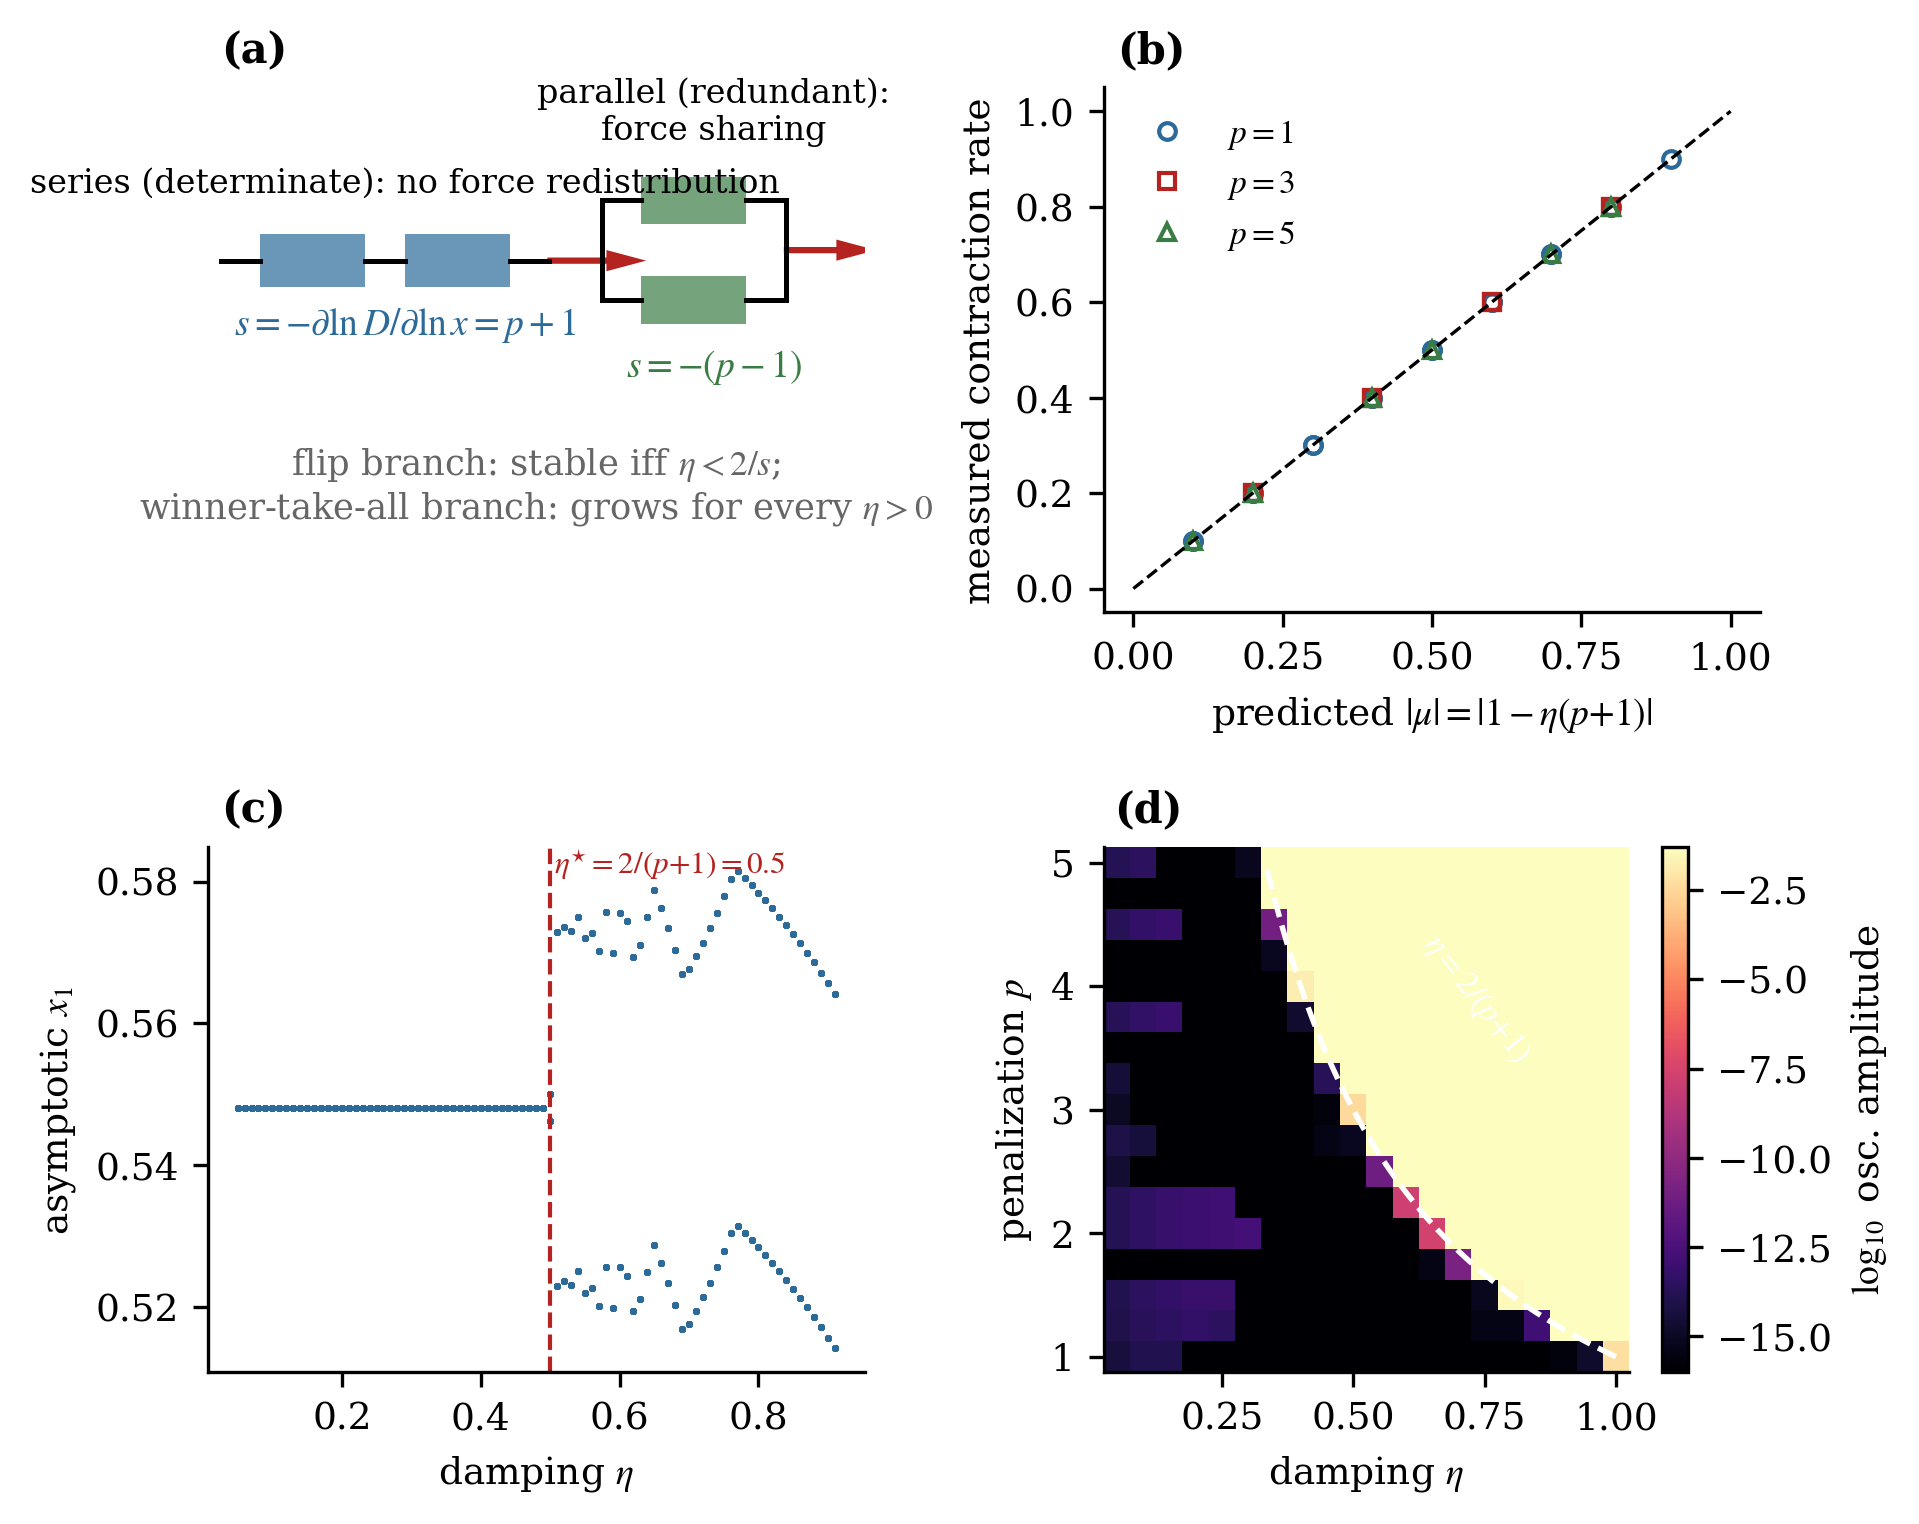
\includegraphics[width=0.86\textwidth]{fig_toy_pub.png}
\caption{The two exact models (Section~\ref{sec:theory}).
(a)~schematic: the series (statically determinate) model carries the
flip branch, $s=p{+}1$; the parallel (redundant) model the
winner-take-all branch, $s=-(p{-}1)$. (b)~measured contraction rates
versus the prediction $|1-\eta(p{+}1)|$ for $p\in\{1,3,5\}$.
(c)~bifurcation diagram at $p=3$ (move limit $0.05$), splitting at
$\eta=0.500$. (d)~oscillation amplitude in the $(\eta,p)$ plane against
the curve $\eta=2/(p{+}1)$.}
\label{fig:toy}
\end{figure}

\begin{figure}[p]
\centering
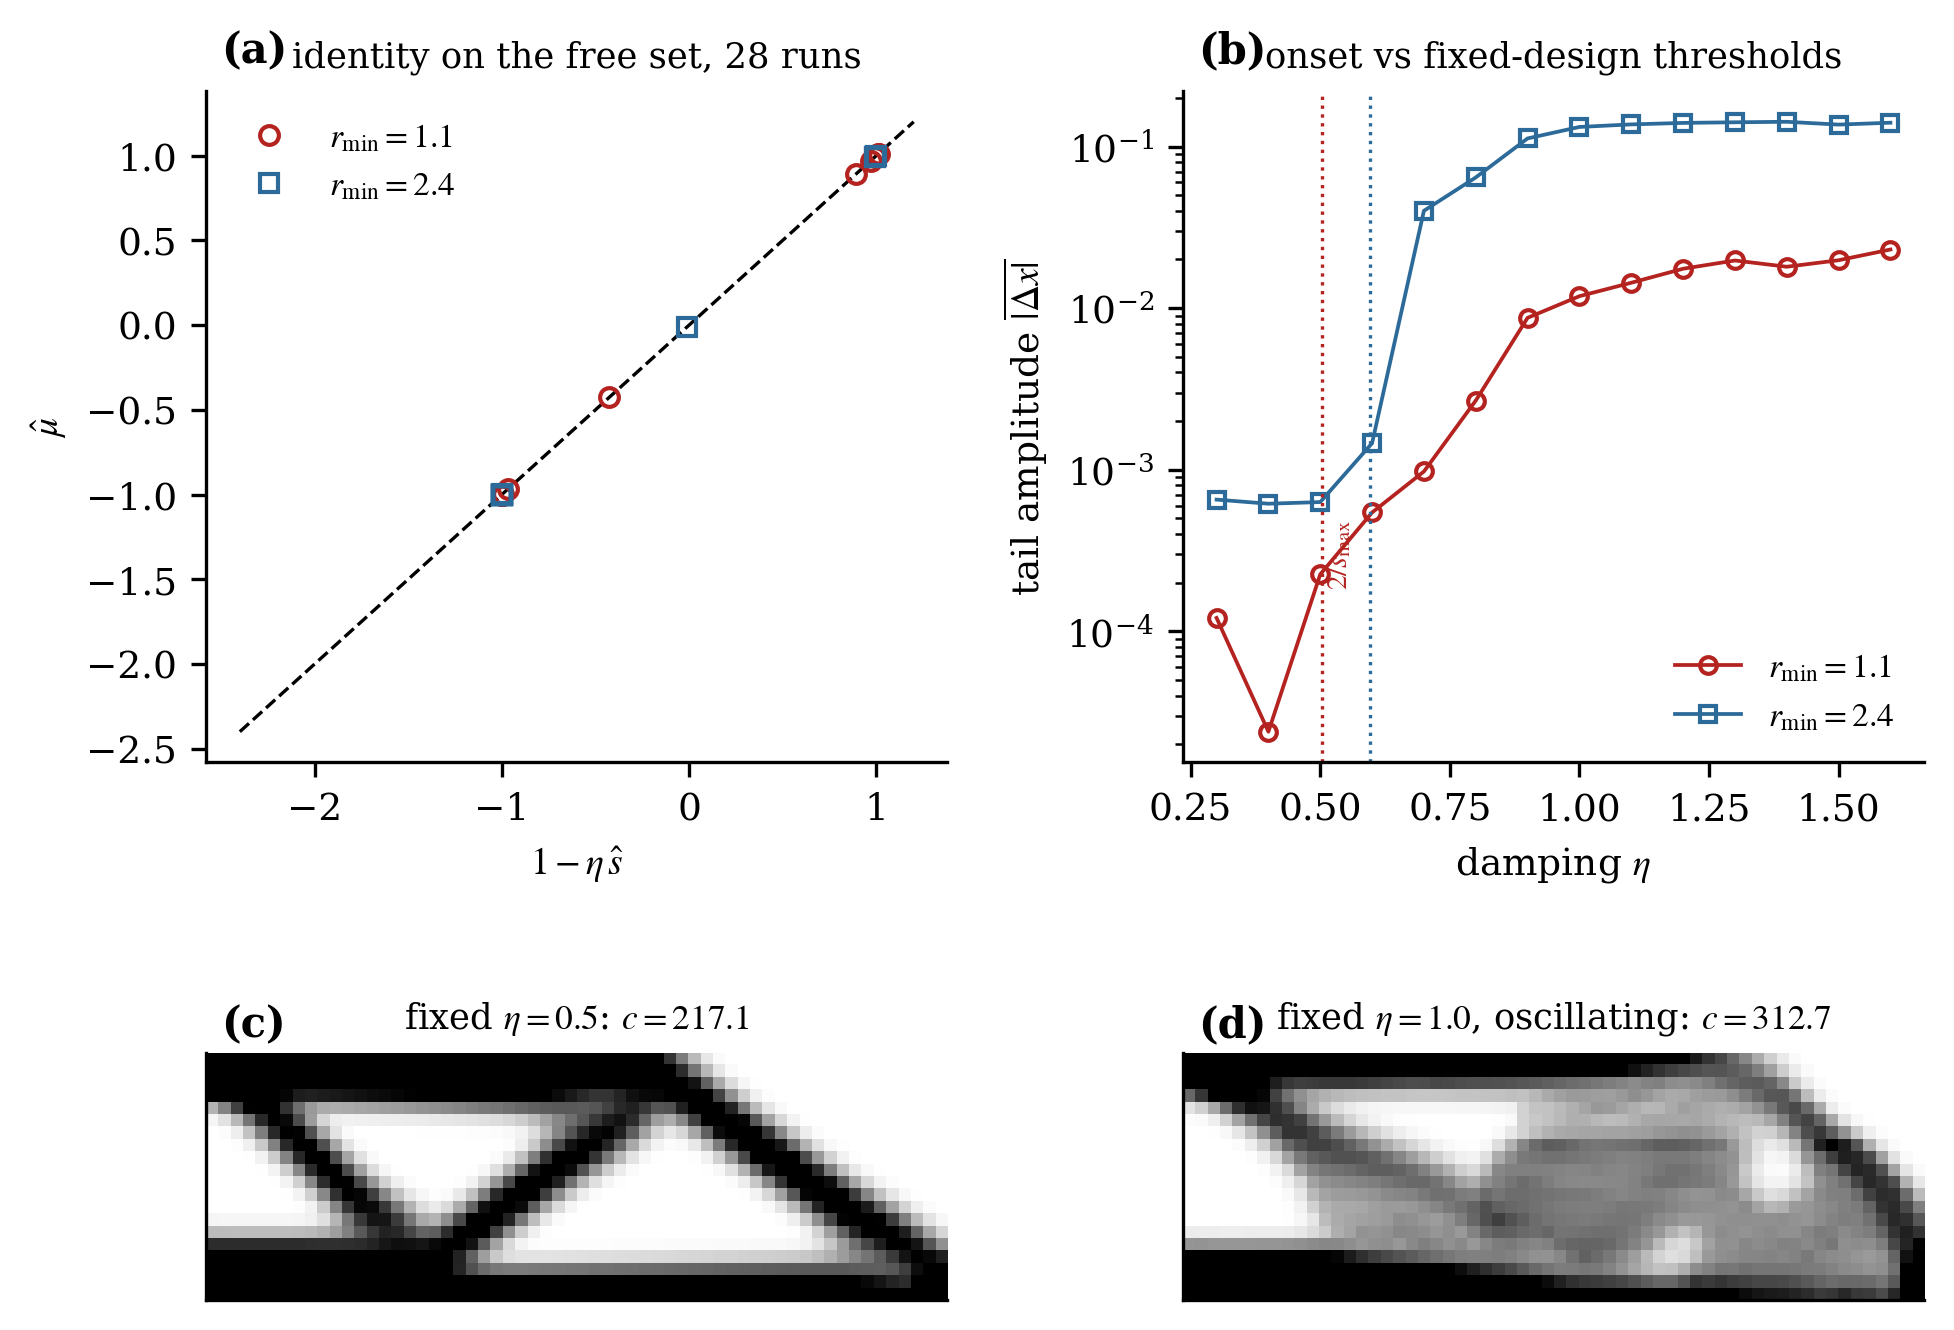
\includegraphics[width=0.86\textwidth]{fig_identity_pub.png}
\caption{Trajectory estimators in the wild
(Section~\ref{sec:validation}). (a)~the identity $\muh=1-\eta\sh$
across the 28-run sweep. (b)~tail amplitude versus $\eta$ at both
filter radii; dotted lines mark the fixed-design thresholds $2/\smax$
($0.503$, $0.596$). (c,d)~converged versus persistently oscillating
designs at $r_{\min}=2.4$ (compliance $217.1$ versus $312.7$ at
$\eta=1.0$, 400 iterations): oscillation is not slow convergence but
lock-in to a damaged design.}
\label{fig:identity}
\end{figure}

\begin{figure}[p]
\centering
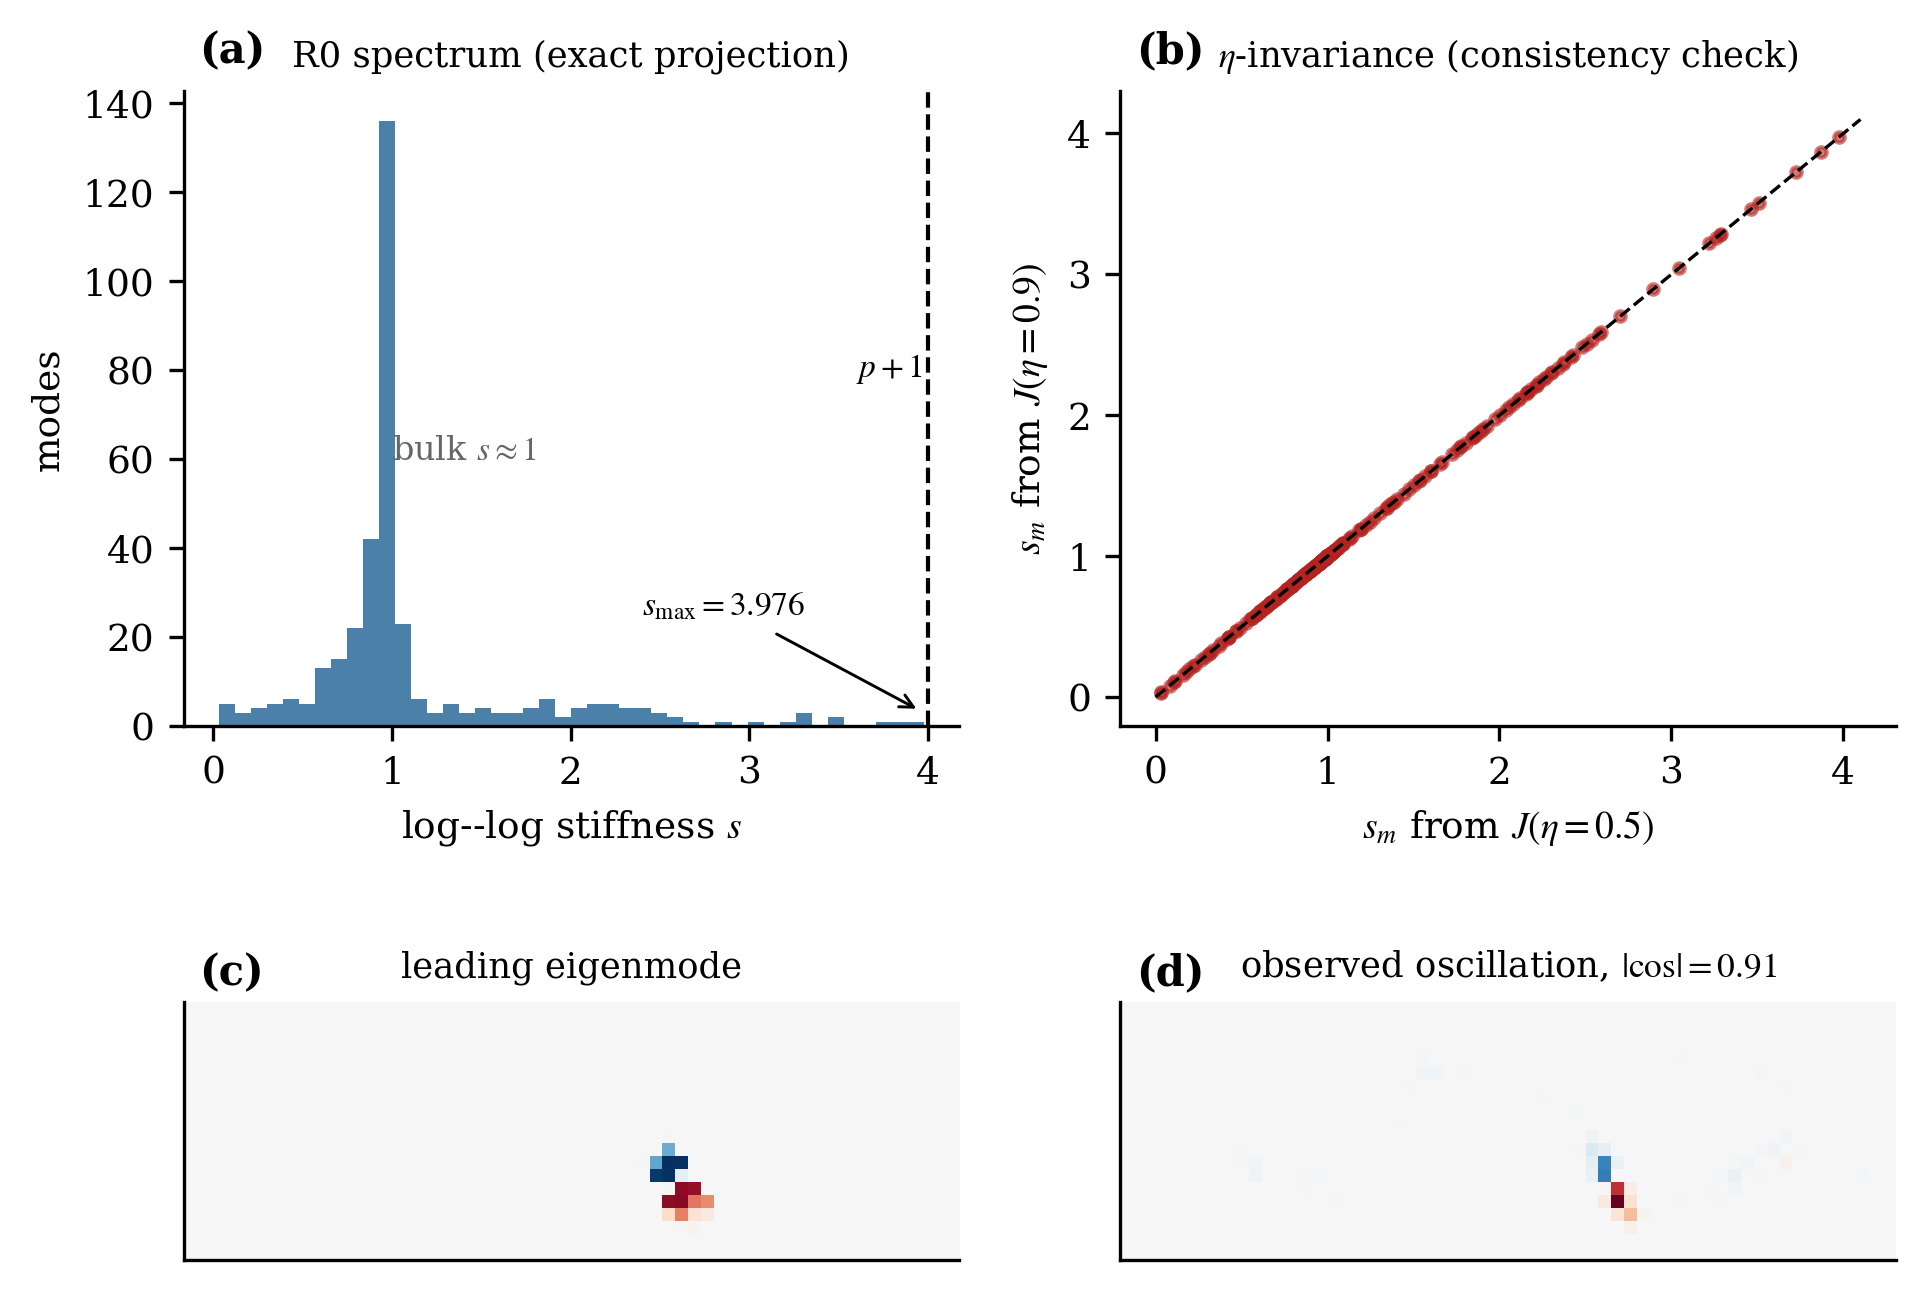
\includegraphics[width=0.86\textwidth]{fig_spectra_pub.png}
\caption{Operator-level spectra at R0
(Section~\ref{sec:validation}). (a)~the exactly projected
$s$-spectrum: bulk at $s\approx1$, lower edge near zero, tail
saturating at $\smax=3.976$ just below $p{+}1$---the shape behind both
the Richardson result and the creep phenomenology. (b)~$\eta$-invariance
of the spectrum (top-five difference $9\times10^{-6}$ between
$J(\eta{=}0.5)$ and $J(\eta{=}0.9)$). (c)~leading eigenmode;
(d)~oscillation pattern measured just above threshold (independent
reproduction, $|\cos|=0.91$; the original measurements give $0.93$ and
$0.96$).}
\label{fig:spectrum}
\end{figure}

\begin{figure}[p]
\centering
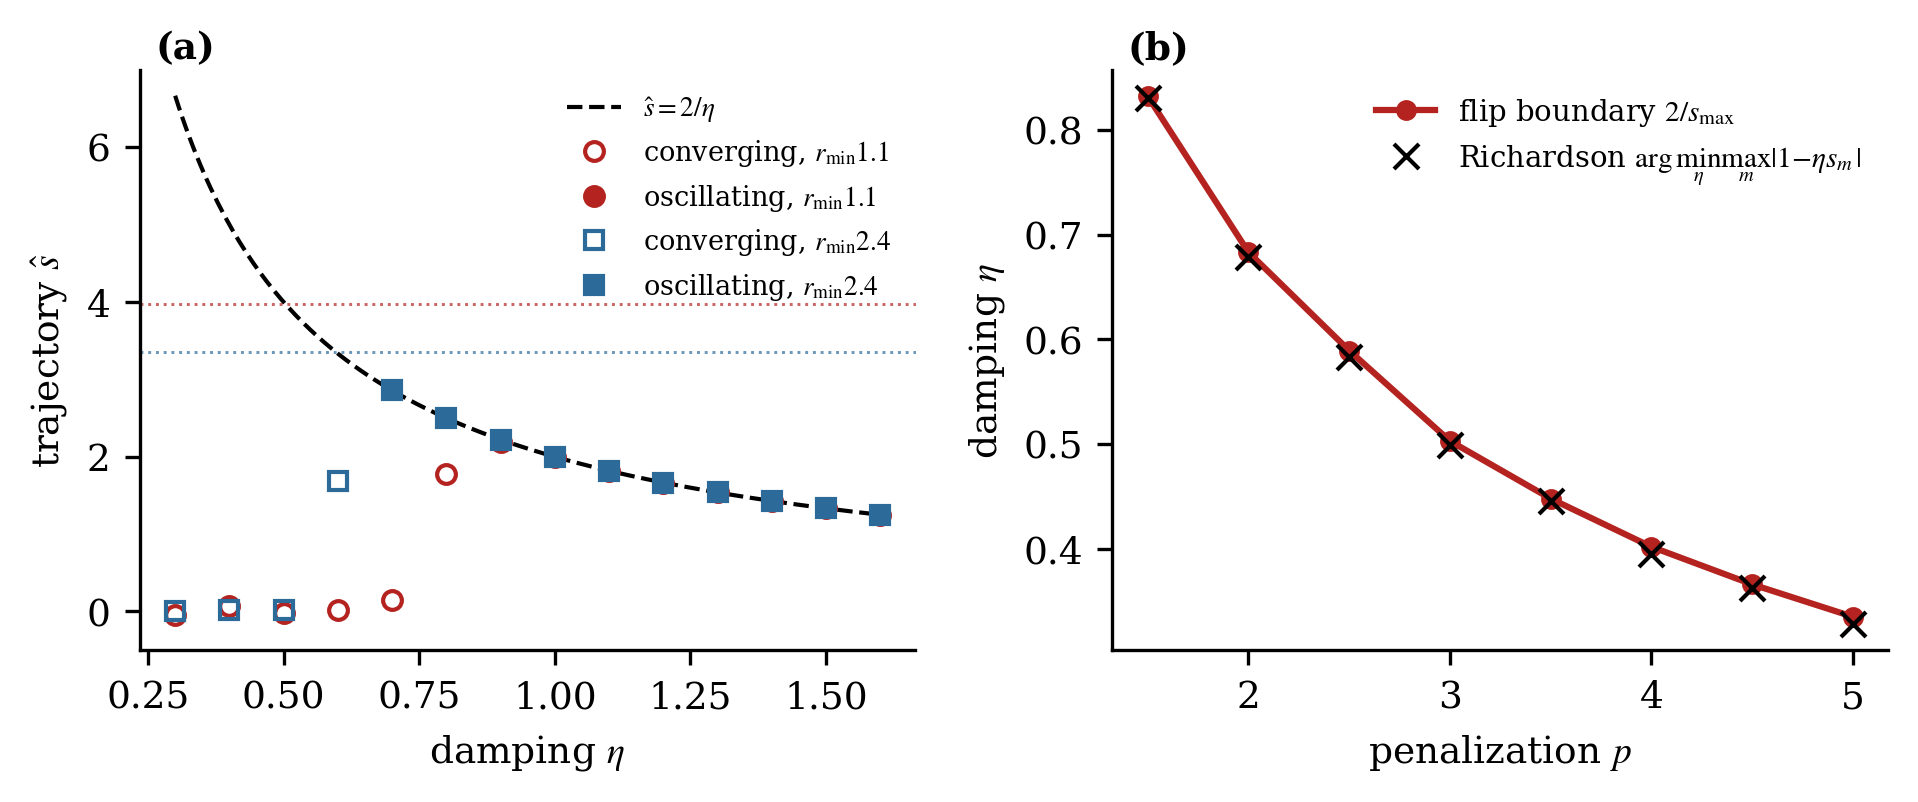
\includegraphics[width=0.92\textwidth]{fig_cycleA.png}
\caption{(a)~The two regimes of the trajectory sensor
(Section~\ref{sec:regimes}): converging runs read the $s\approx0$ creep
edge; saturated runs lock onto $\sh=2/\eta$; dotted lines mark operator
$\smax$. (b)~The min--max optimal damping coincides with the flip
boundary across the penalization sweep
(Section~\ref{sec:richardson}).}
\label{fig:gate}
\end{figure}

\begin{figure}[p]
\centering
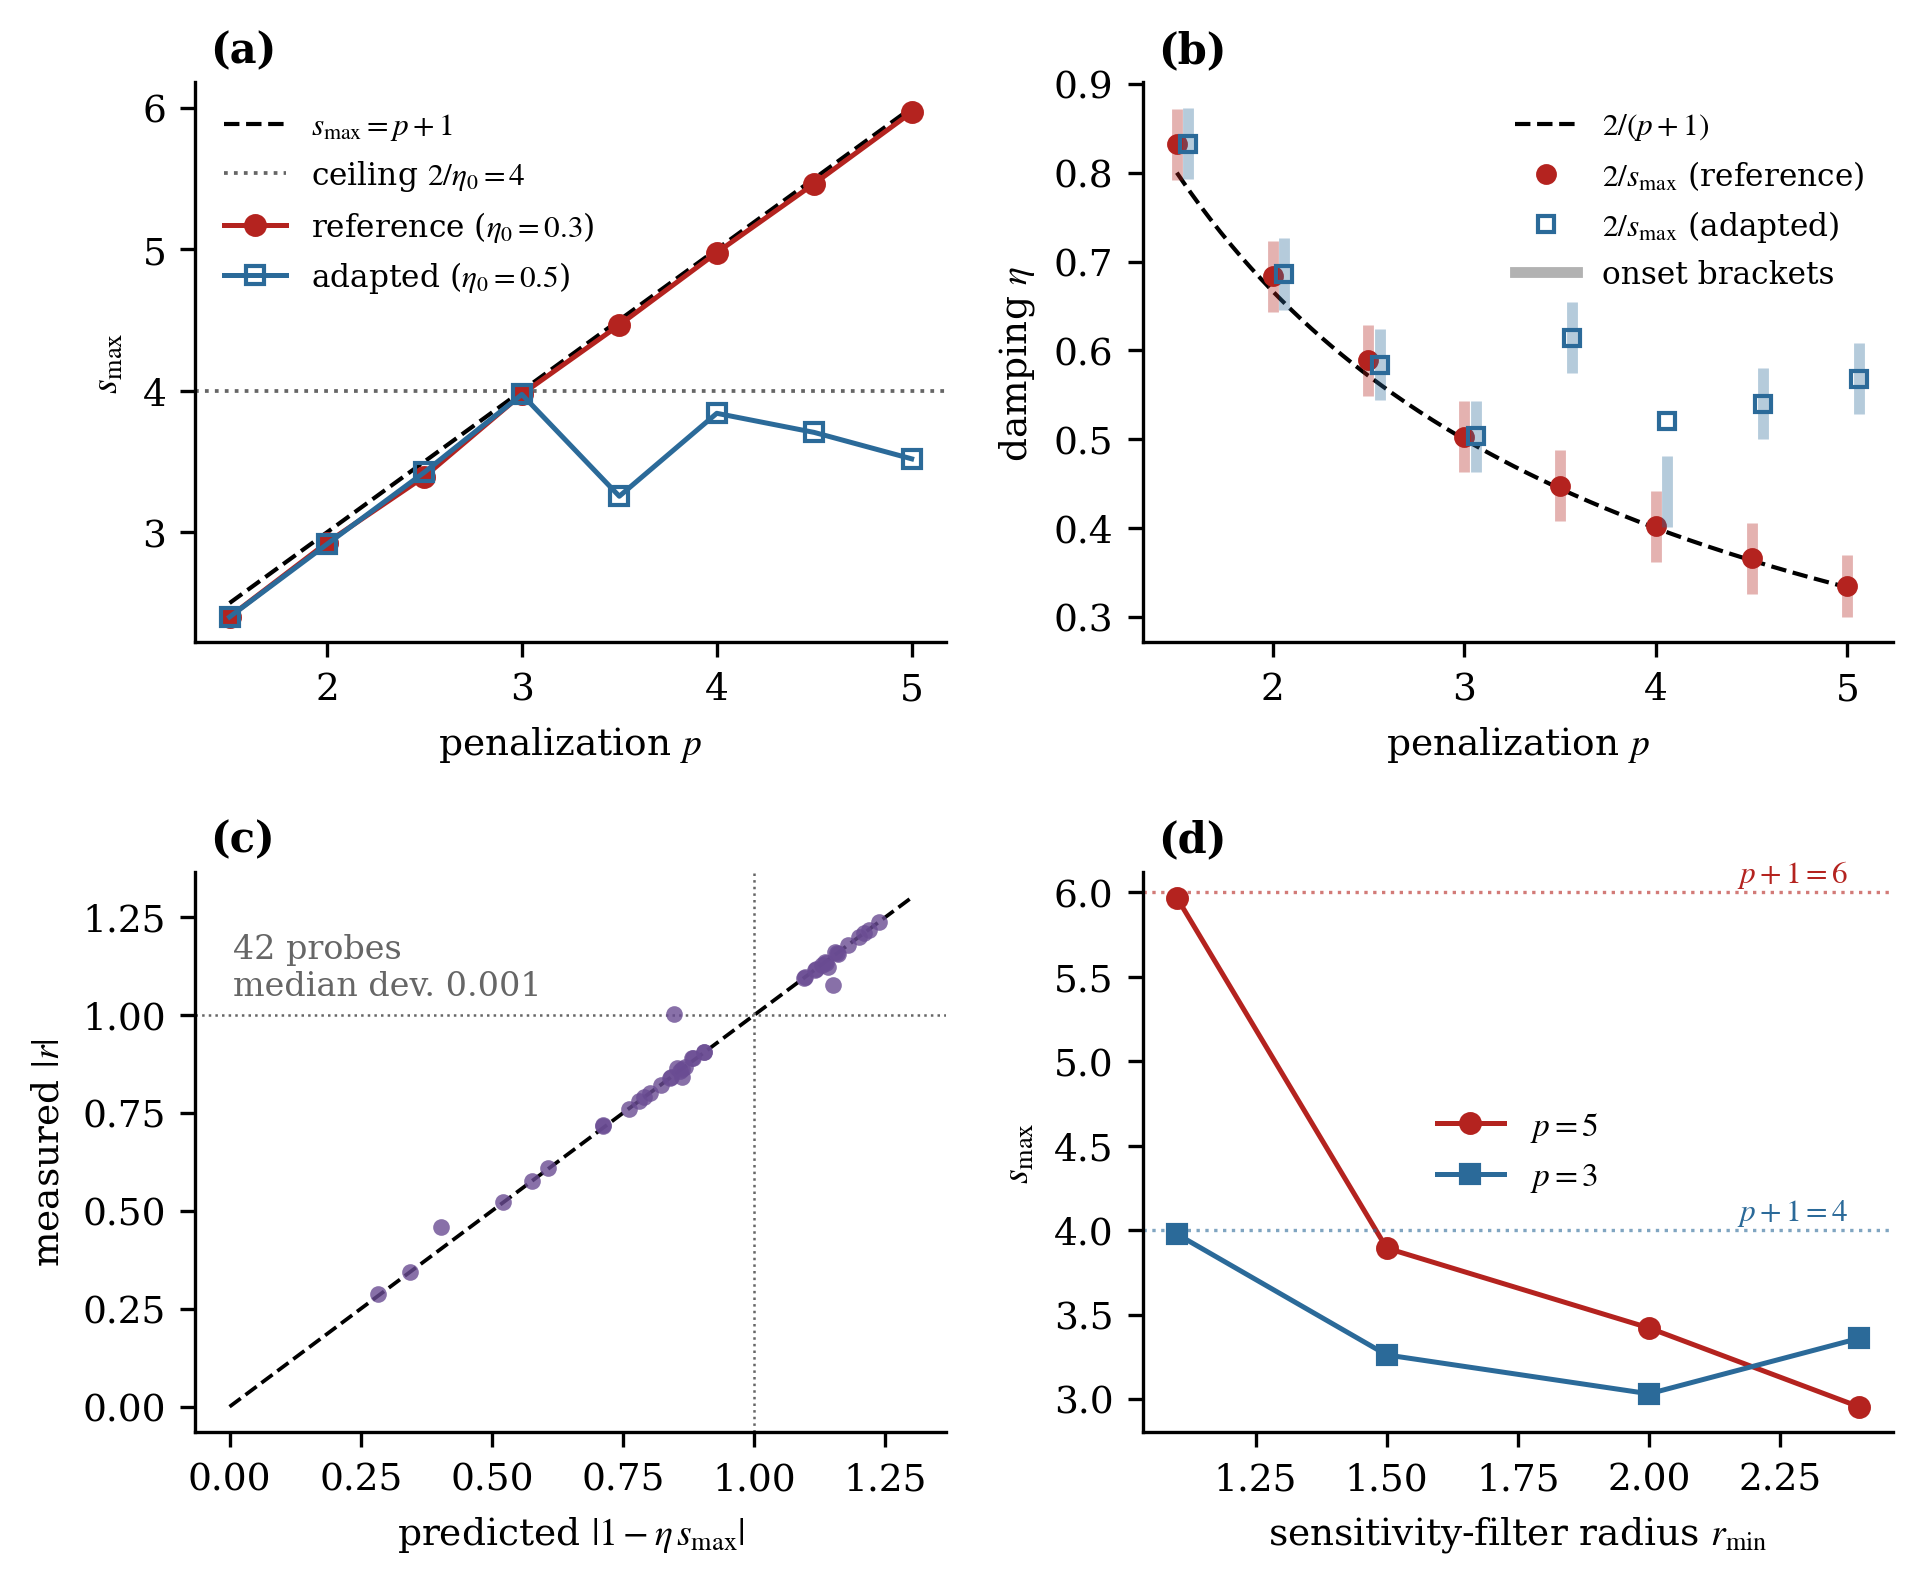
\includegraphics[width=0.92\textwidth]{fig_psweep_pub.png}
\caption{Penalization sweep (Section~\ref{sec:saturation}):
saturation under the reference protocol versus self-limiting under
standard damping, separating at $p=3$; onset brackets following each
fixed point's own $2/\smax$; the rate law across both protocols;
filter-radius detuning.}
\label{fig:psweep}
\end{figure}

\begin{figure}[p]
\centering
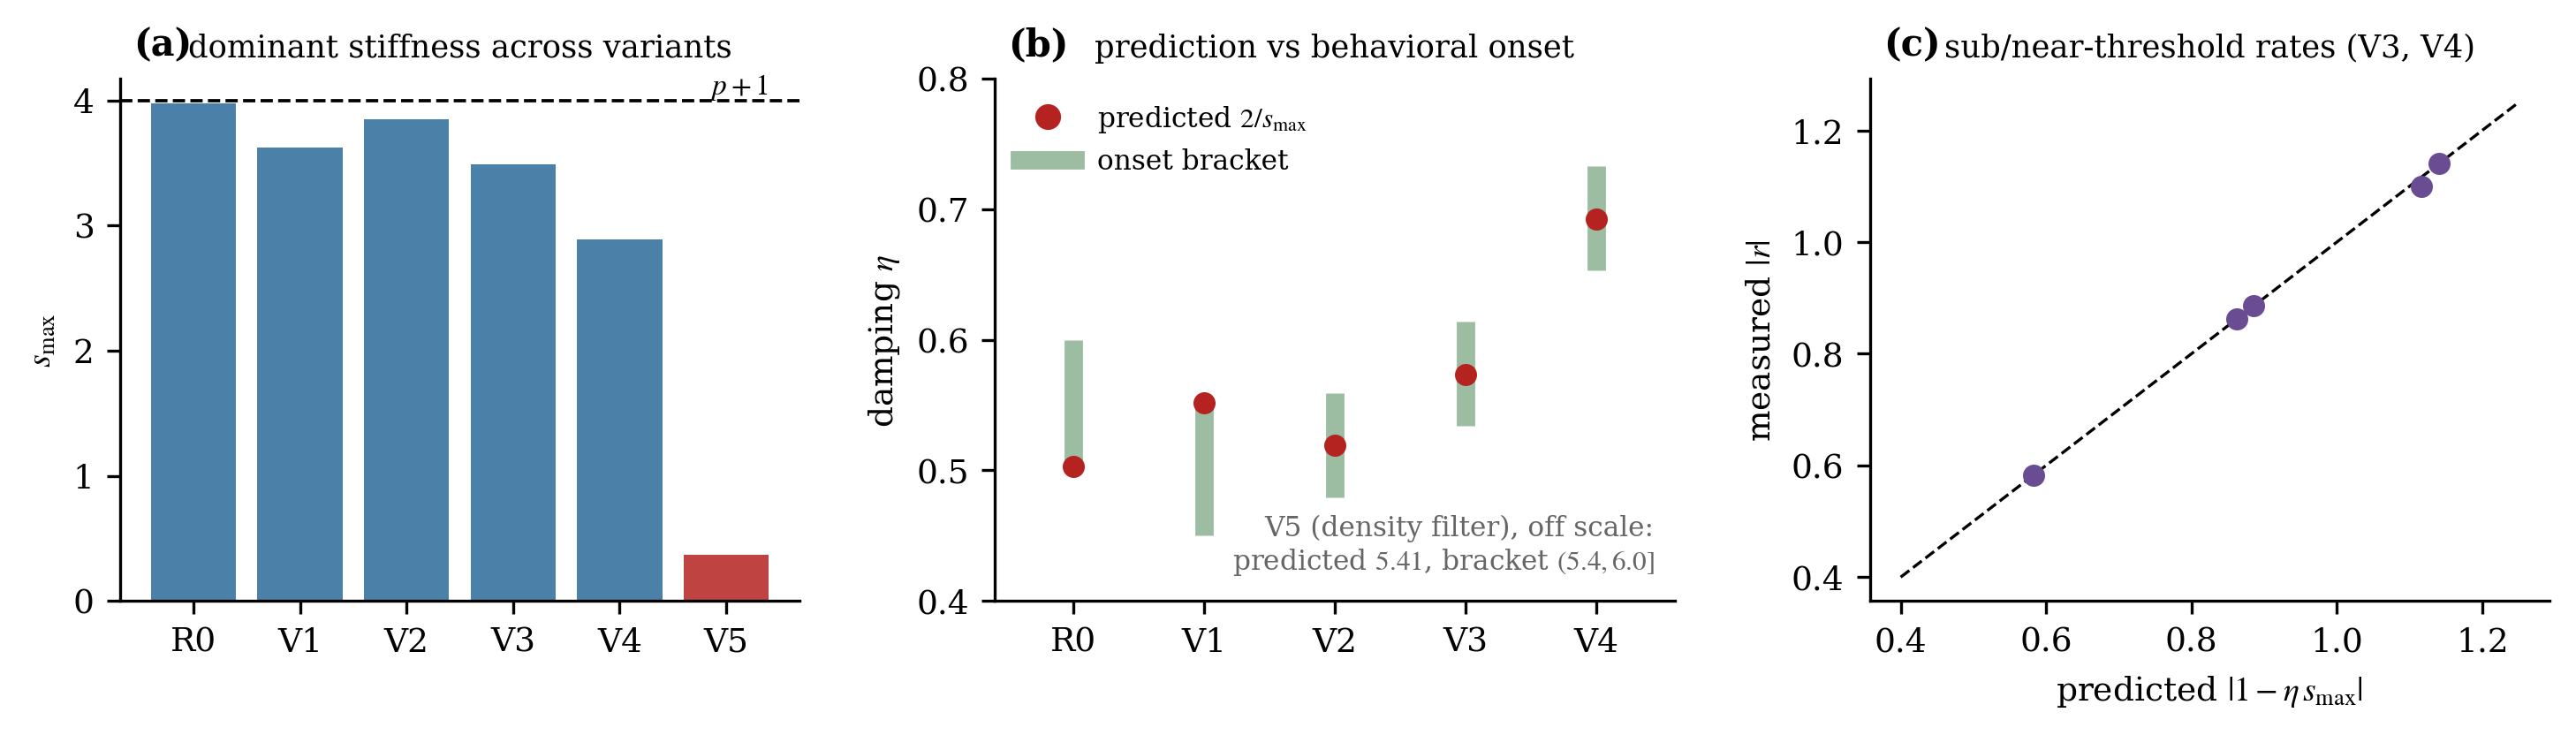
\includegraphics[width=\textwidth]{fig_robust_pub.png}
\caption{Robustness of the threshold law (Section~\ref{sec:validation},
Table~\ref{tab:robust}). (a)~$\smax$ across variants; the density
filter (V5) collapses it to $0.37$. (b)~predicted $2/\smax$ versus
behavioral onset brackets for R0--V4 (V5 off scale: predicted $5.41$,
bracket $(5.4,6.0]$). (c)~flip-active probe rates versus
$|1-\eta\,\smax|$ on V3/V4---three-decimal agreement below threshold.}
\label{fig:robust}
\end{figure}

\begin{figure}[p]
\centering
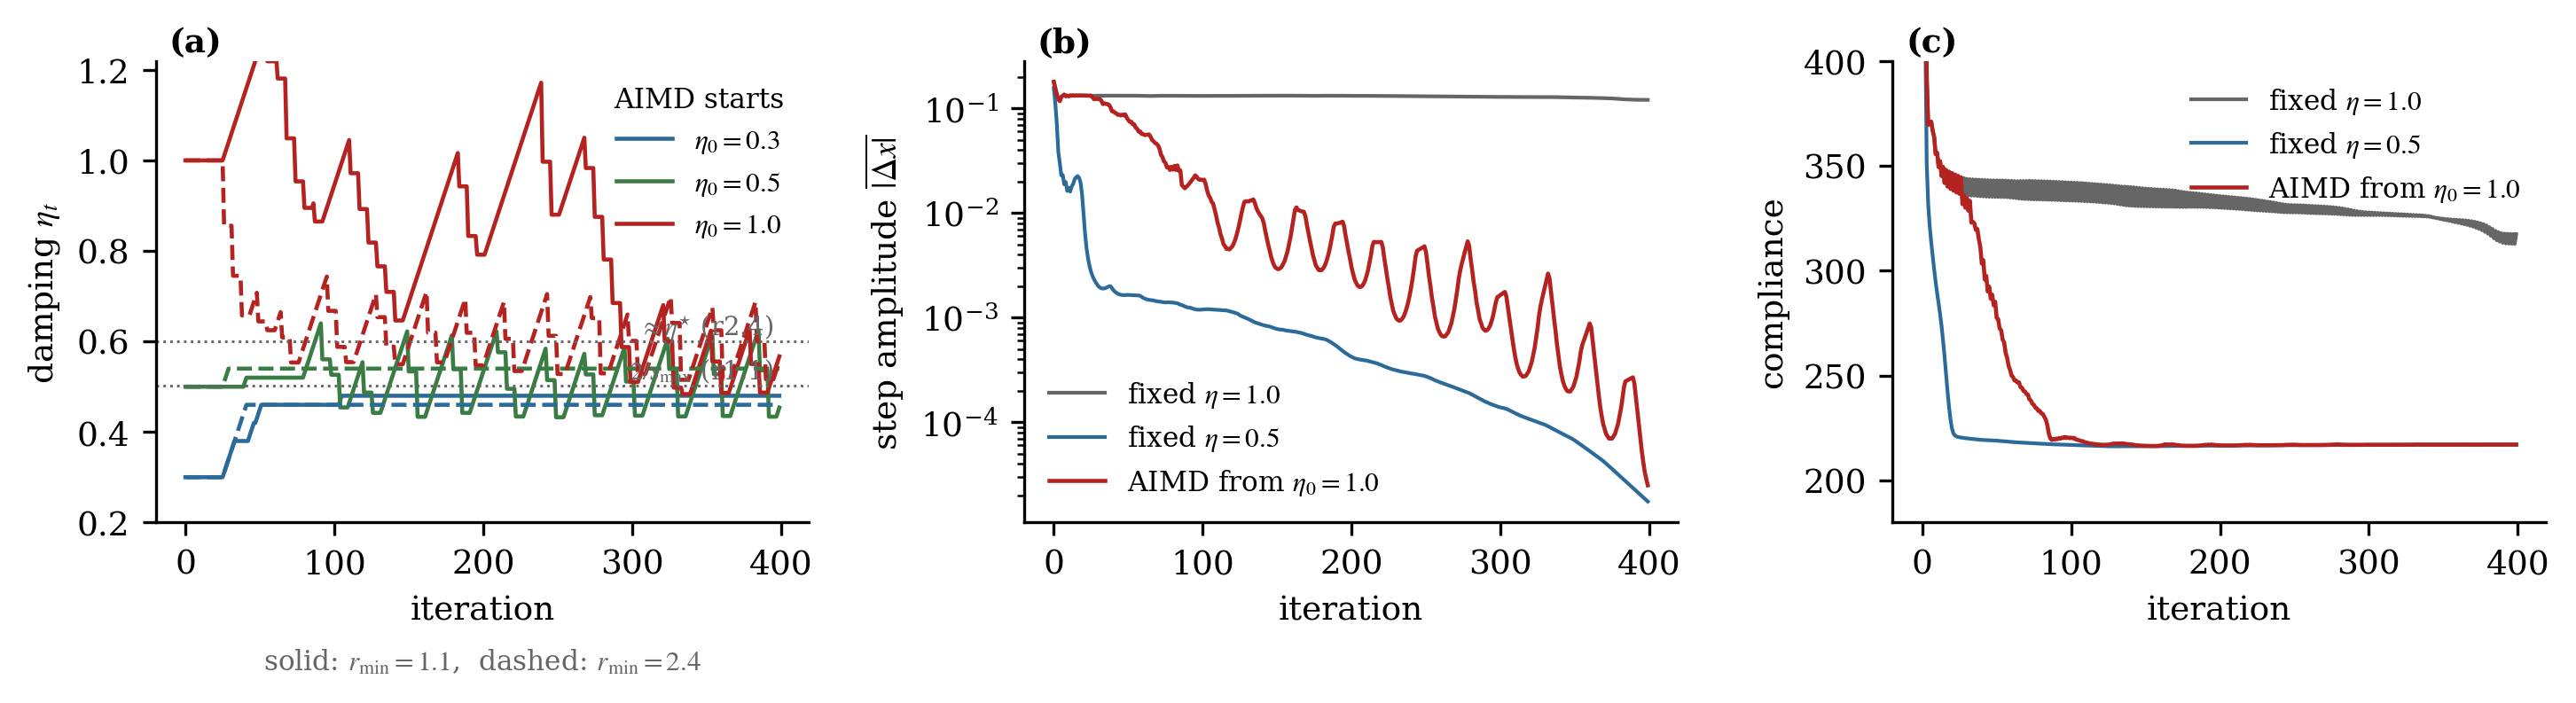
\includegraphics[width=\textwidth]{fig_cycleB.png}
\caption{The controller on two problems from three starts
(Section~\ref{sec:demos}): damping trajectories landing in each
problem's own threshold band; rescue of the over-driven hard-filter run;
compliance recovery.}
\label{fig:aimd}
\end{figure}

\begin{figure}[p]
\centering
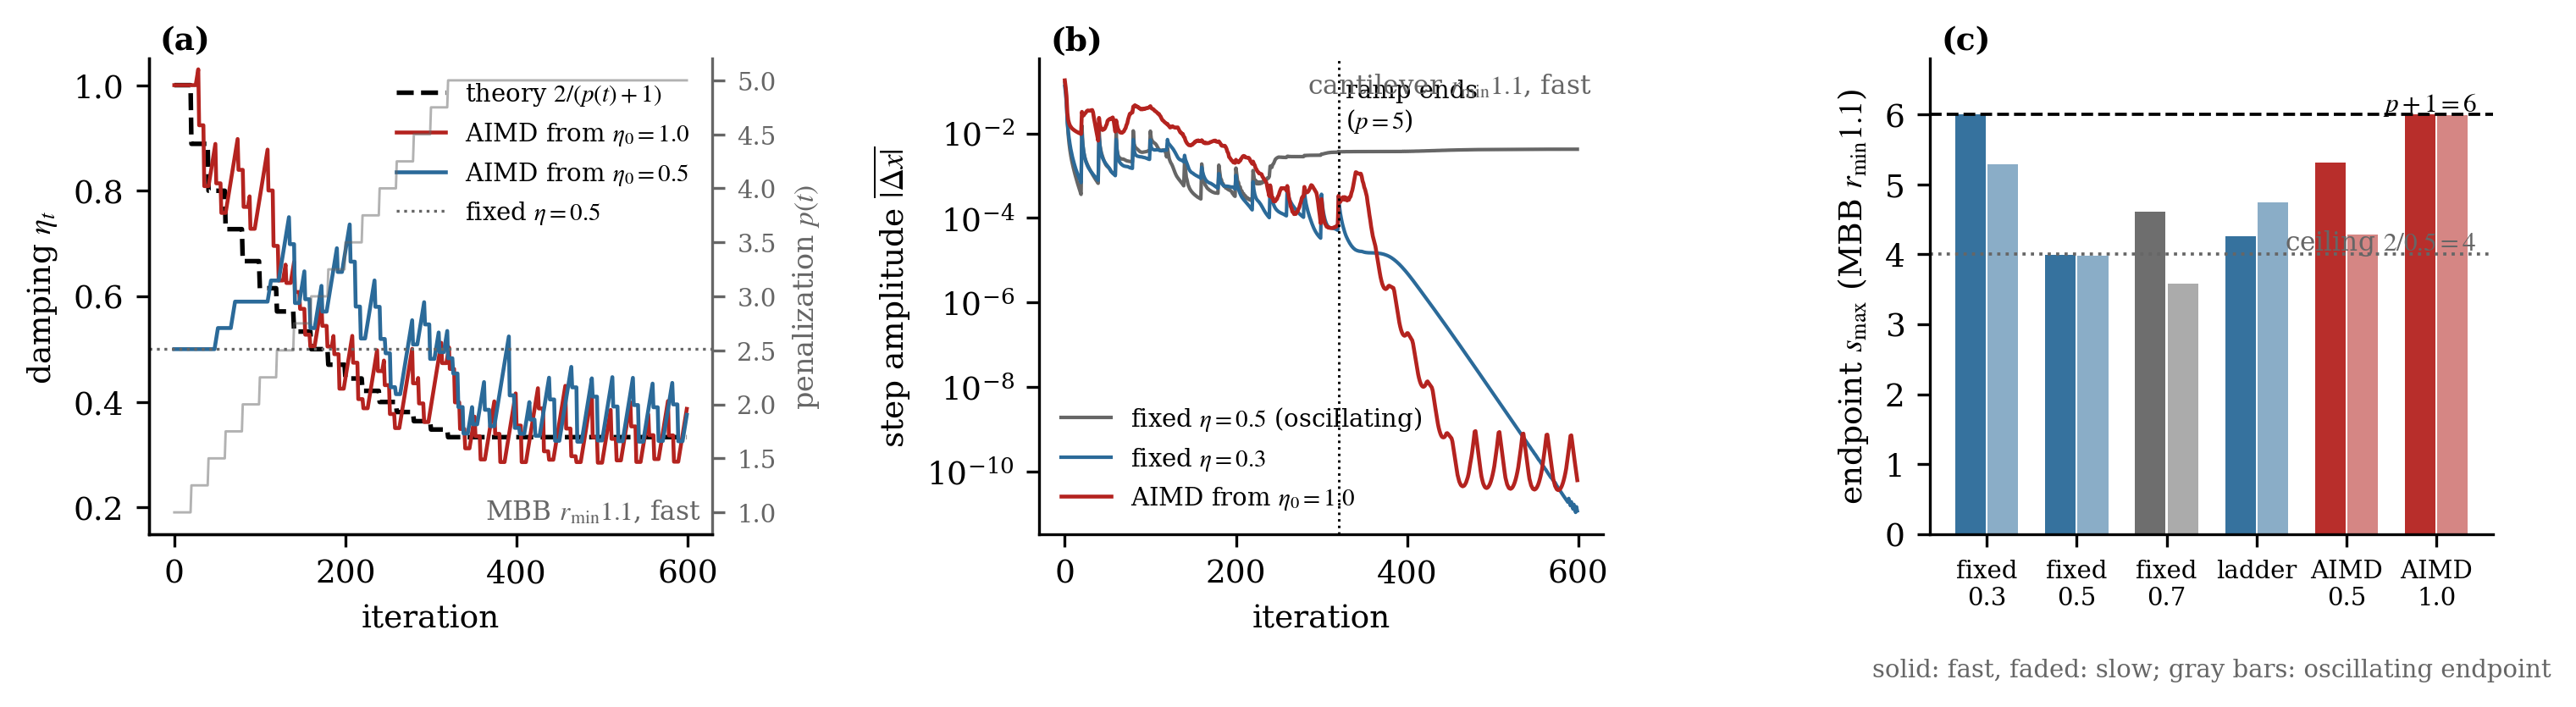
\includegraphics[width=\textwidth]{fig_cont.png}
\caption{Penalization continuation ($p:1\to5$;
Section~\ref{sec:continuation}). (a)~the controller's damping tracks the
falling threshold $2/(p(t){+}1)$ it was never told about (MBB
$r_{\min}1.1$, fast schedule; right axis: $p(t)$). (b)~the fast ramp
breaks fixed $\eta=0.5$ on the cantilever while the controller converges
to $10^{-10}$. (c)~endpoint $\smax$: fixed $0.5$ lands on the capacity
ceiling $2/\eta=4$, the controller from $\eta_0=1.0$ reaches the
naturally saturated family $p{+}1=6$, on both schedules.}
\label{fig:cont}
\end{figure}

\begin{figure}[p]
\centering
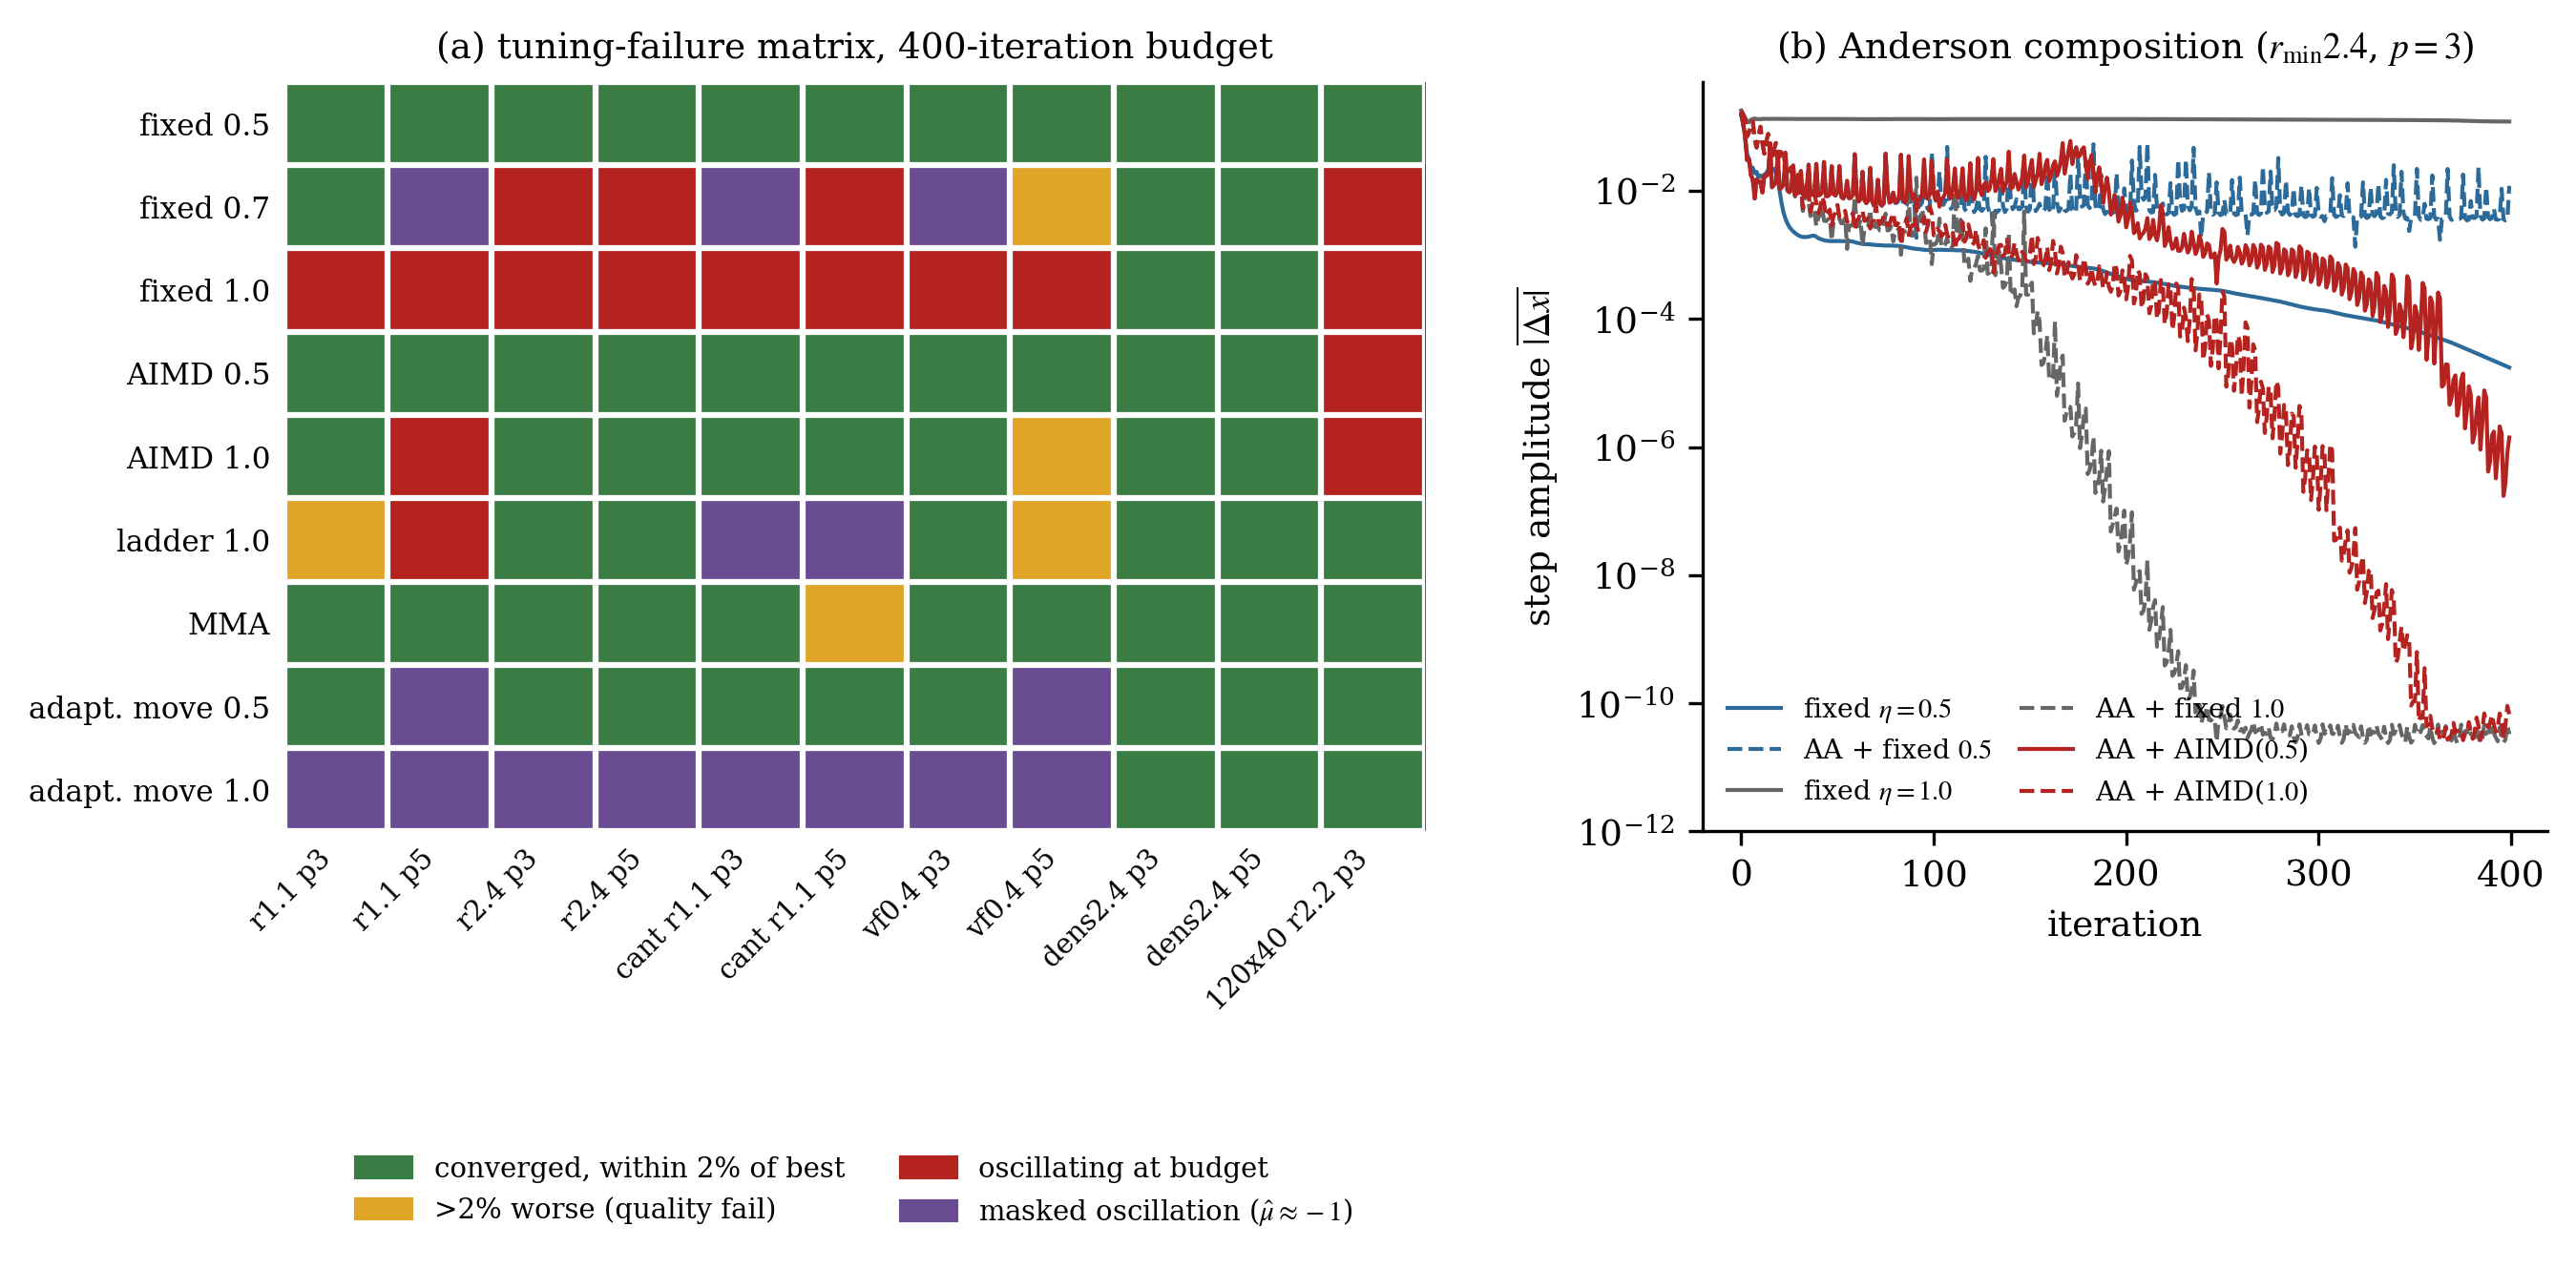
\includegraphics[width=\textwidth]{fig_cycleC.png}
\caption{(a)~Tuning-failure matrix across the 11-group suite
(Section~\ref{sec:sweeprates}). (b)~Anderson composition
(Section~\ref{sec:anderson}): AA breaks the well-tuned run and fixes the
over-driven one; the composition with the controller converges deepest
from both starts.}
\label{fig:failmatrix}
\end{figure}

\begin{figure}[p]
\centering
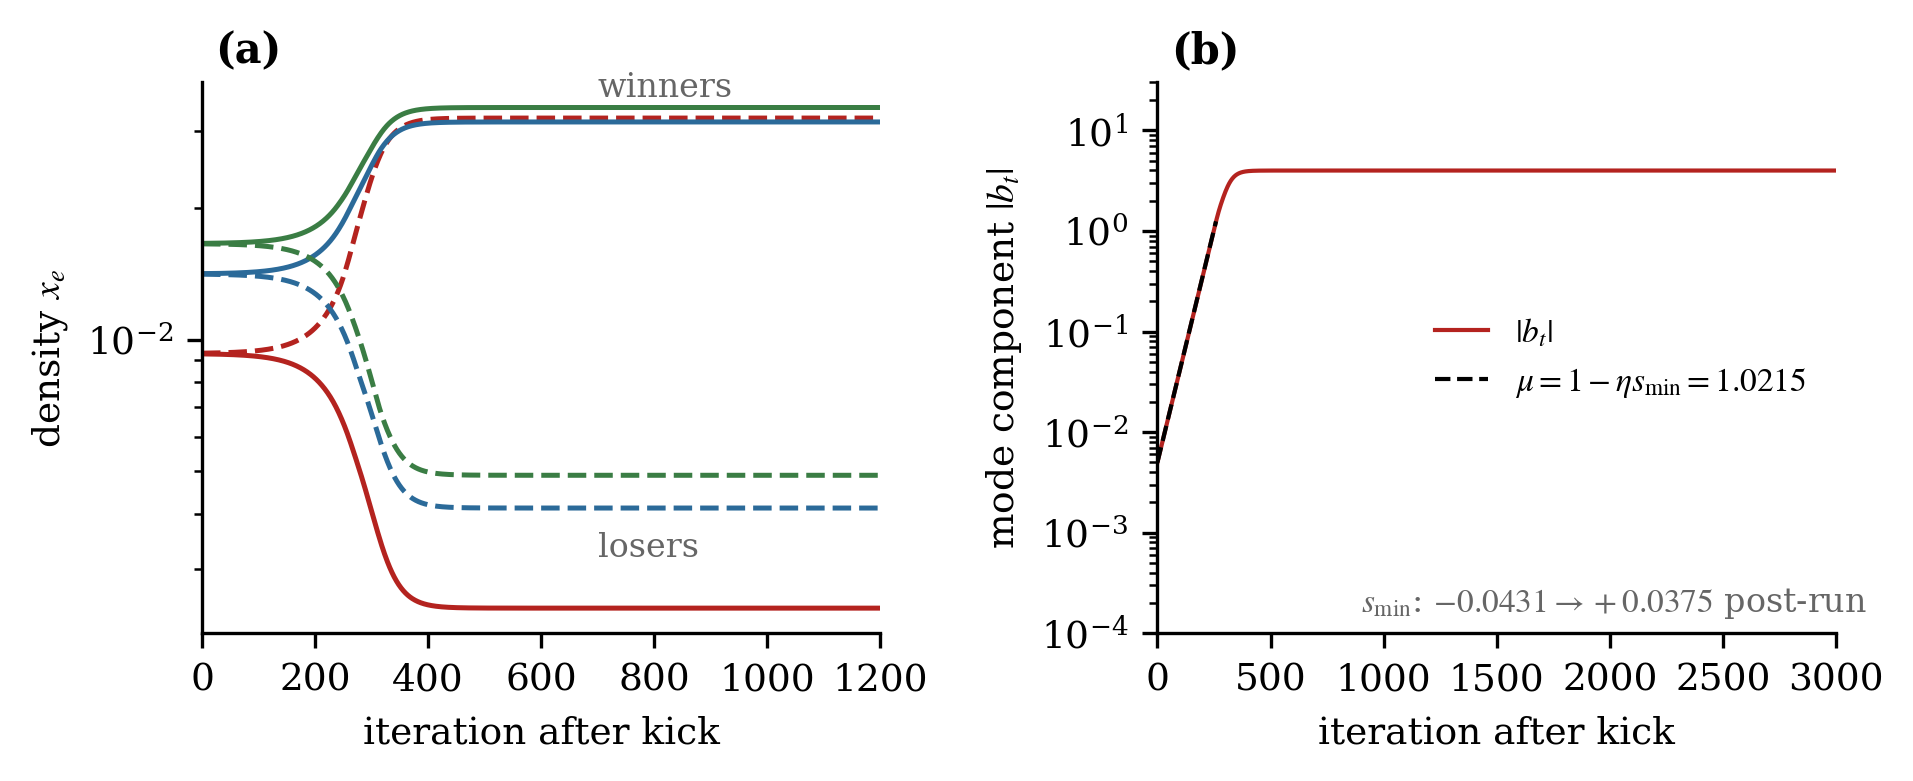
\includegraphics[width=0.92\textwidth]{fig_negbranch.png}
\caption{Appendix~\ref{app:neg}: mirror-pair symmetry breaking of the
negative branch and growth at the predicted rate, terminating in an
asymmetric fixed point.}
\label{fig:negbranch}
\end{figure}

\bibliographystyle{plainnat}
\bibliography{refs}

\end{document}
